\documentclass[11pt, oneside]{book}
\usepackage[utf8]{inputenc}
\usepackage{lmodern}
\usepackage[T1]{fontenc}
\usepackage{amsmath, amssymb, amsthm}
\usepackage{graphicx}
\usepackage{tikz}
\usepackage{hyperref}
\usepackage{geometry}
\usepackage{xcolor}
\usepackage{natbib}
\usepackage{hyperref}
\usepackage{macros}
\usepackage{enumitem}
\geometry{margin=1in}

\newcounter{exercise}
\newenvironment{exercise}[1][]{%
    \par\medskip\refstepcounter{exercise}%
    \noindent\textbf{Exercise \theexercise.}\ \textit{#1}\par\nopagebreak\medskip%
}{\par\medskip}

% \title{\textbf{Physics 198: Learning Mechanics \\
% \large Course Notes}}
% \date{UC Berkeley}
% \author{Mark Rhee}

\begin{document}
% \maketitle

\begin{titlepage}
\newgeometry{top=2in, bottom=1in, left=1in, right=1in}
\raggedright
 
\vspace*{2cm}
{\fontsize{32}{40}\selectfont\bfseries Learning Mechanics}\\[0.6em]
{\fontsize{20}{28}\selectfont\bfseries Course Notes}
 
\vspace{2.5cm}
 
{\large Mark Rhee}
 
\vfill
 
\restoregeometry
\end{titlepage}

\chapter{Introduction to Neural Networks}
Deep learning is in a peculiar situation at this moment in time. Empirically, the capabilities of AI leveraging deep learning (eg. LLMs) have surpassed the expectations of even the most radically optimistic researchers. Publicly available LLMs are \href{https://x.com/__alpoge__/status/2079028340955197566}{disproving math conjectures} left and right, AI is being \href{https://icml.cc/virtual/2026/invited-talk/67266}{injected into every stage of real drug development life cycles}, \href{https://tinyurl.com/2hhcsnz7}{entire business models have been destroyed} by improving AI capabilities, and at this point, AI \href{https://www.nobelprize.org/prizes/chemistry/2024/press-release/}{winning a Nobel Prize} is old news. Yet, we lack a comprehensive scientific framework for understanding 
how exactly these models work and the development of frontier models is closer to alchemy than science.

Not long ago, engineers built working steam engines before anyone understood the science behind them. The effort to understand and build better engines ended up creating an entirely new branch of science: statistical mechanics. Deep learning may be our generation's steam engine. \textit{Learning mechanics} is the emerging discipline that aims to understand it from first principles, treating deep learning the way physics treats the natural world: seeking compact mathematical principles, tight connections between theory and experiment, and simple, intuitive explanations for complex phenomena.

% In 2024, one half of the Nobel Prize in Chemistry was awarded to Demis Hassabis and John Jumper of Google DeepMind for developing AlphaFold---an AI model that predicts protein structures form amino acid sequences. Despite this monumental achievement, the \textit{protein folding problem} remains unsolved; that is, we still lack a first-principles understanding of how protein structures emerge from a linear sequences of amino acid residues\footnote{Source: https://www.pnas.org/doi/10.1073/pnas.2214423119}. It turns out, training a model to predict does not necessarily mean we will comprehend how it predicts.

% The same problem persists with Large Langauge Models (LLMs). As of 2026, frontier labs have spent hundreds of billions of dollars scaling LLMs, guided more or less by an empirical observation: that more compute, more data, and more parameters seem to produce better models. By some estimates, data center investment now accounts for roughly half of U.S. GDP growth, surpassing total consumer spending as a share of the economy\footnote{Source: https://americanaffairsjournal.org/2026/02/understanding-the-llm-bubble/}. And yet ask any honest AI researcher and they will tell you that we have barely scratched the surface in terms of understanding \textit{why} or \textit{how} any of this works. 

% \textcolor{red}{TODO} Building powerful AI that we don't understand well is dangerous. A potential problem is that even if there is sufficient political will to regulate, without a scientific understanding of its inner workings, we may lack the technical language to regulate it properly.

% In both cases, capabilities have far out-paced comprehension. We can build these systems, deploy them, stake a Nobel Prize or a national economy on them, yet we cannot explain why they work or what they have learned. This is the practical motivation for \textit{learning mechanics}. That being said, beyond the practical stakes, the astounding empirical success of deep learning is also a genuine scientific mystery that should spark our curiosity. The ingredients for deep learning are remarkably simple, yet the results are not. Understanding how deep learning works would reshape our understanding of intelligence itself: how structure emerges from data, why certain neural representations arise, how representations are used for computation, and what it even means to learn.

% \textit{A note on scope.} Deep learning has a long and intricate history, and the literature surrounding even the simple setup we are about to introduce is vast---spanning decades of work on architectures, optimization, and theory. This chapter (and for the most part, the chapters that follow) deliberately sets nearly all of it aside. The goal here is not a survey but an \textit{on-ramp}: the most direct route to the questions and tools of learning mechanics. We will introduce only what we need, when we need it.

% \textit{A note on a sister-field.} The field of \textit{mechanistic interpretability} aims to understand how complex models work by identifying structures, circuits or algorithms embedded in the weights of the models. The motivations and goals for the field are nearly identical to that of learning mechanics; the differences lie in methodology and the resolution at which each field aims to understand models. The following quote is from the perspective paper that introduced learning mechanics\footnote{Source: https://arxiv.org/pdf/2604.21691}.

% \begin{quote}
%     "Where mechanistic interpretability aims to be the biology of deep learning, learning mechanics should aspire to be its physics, mirroring the complementary relationship between biology and physics in the natural sciences."
% \end{quote}

% We will not cover mechanistic interpretability in depth, but in later chapters, we will see the symbiotic relationship between the two fields in action.

\section{Deep Neural Networks}

At the heart of modern machine learning are \textit{deep neural networks}. Nearly every headline-grabbing AI system of the past decade (AlphaGo, GPT, AlphaFold, Stable Diffusion, etc.) is, at its core, a deep neural network trained by gradient descent on a large dataset---or some other similar architecture that heavily relies on deep neural networks. If we want a scientific theory of modern AI, we need a scientific theory of neural networks.

\subsection{The deceptively simple setup}

Consider a standard supervised learning task. We are presented with $P$ pairs of data points $\{ (x_{i}, y_{i}) \}_{i=1}^P$, each consisting of an input vector $x_i$ and an output vector $y_i$. 
We assume that the inputs $x$ are sampled from some data distribution $x\sim \rho$, and
the outputs $y$ are generated by some target function $y=f^*(x)$.
We "learn" a function $\hat{f}$, i.e., a model, such that $\hat{f}(x_{i}) \approx f^*(x_i) = y_{i}$ for all $i = 1, \dots, P$. 
The goal is to learn a "good" model $\hat{f}$ such that it agrees with $f^*$ on
the entire data distribution $\rho$ instead of just on the $P$ sampled data points.
The canonical example of a supervised learning task is that of handwritten digit recognition. Here, each input $x\in \mathbb{R}^d$ is a flattened image of a handwritten digit, where $d$ is the number of pixels and each element records the intensity of the corresponding pixel. The output vector $y\in\mathbb{R}^{10}$ corresponding to $x$ is a one-hot vector indicating which digit (0, 1, \dots, 9) the image depicts. The goal is to learn a function $\hat{f}$ that maps raw pixel intensities to the correct digit.

A neural network is a particularly powerful choice of model. In its simplest form, it applies a linear transformation to the input and then passes the result through a \textit{point-wise nonlinearity} $\sigma$, e.g., a Rectified Linear Unit (ReLU):

\begin{equation}
    \hat{f}(x)=\sigma(Wx).
\end{equation}

Since the composition of linear transformation and nonlinearity occurs only once, we say this network has 1 layer. Stacking $L$ such operations yields a \textit{deep} neural network:

\begin{equation}
\hat{f}(x)=W_{L}(\sigma(W_{L-1}\sigma(\dots \sigma(W_{1}x)))).
\label{dnn}
\end{equation}

So now we have the \textit{architecture}, but how shall we set the values of the weight matrices $W_1, \dots,W_L$? The answer is that we will \textit{learn} them through a process called \textit{training}.

Training consists of minimizing a \textit{loss function}, e.g., Mean Squared Error (MSE):

\begin{equation}
\mathcal{L}_{\text{MSE}}(\mathbf{\theta}) = \sum^P_{i=1}||y_{i}-\hat{f}(x_{i})||^2.
\label{mse}
\end{equation}

We minimize the loss function by \textit{randomly initializing} the weight matrices and updating them through \textit{Gradient Descent (GD)}:

\begin{equation}
W_{l} \leftarrow W_{l}-\eta \nabla_{W_{l}} \mathcal{L}
\label{gd}
\end{equation}

where $\theta$ represents the learnable parameters in the model (the elements of the weight matrices in this case) and $\eta$ is some small positive number called the \textit{learning rate}.

That's it. That's pretty much the whole setup: an \textbf{architecture}, some \textbf{data}, a \textbf{loss function}, and a \textbf{learning rule}. Granted, practitioners have learned to add various bells and whistles to this simple setup to get everything to work in the real-world. On the architectural side, modern networks incorporate residual connections, convolutional blocks, and attention mechanisms. On the learning rule side, vanilla gradient descent is typically replaced by minibatch variants such as Stochastic Gradient Descent (SGD) or more sophisticated optimizers like Adam or Muon and regularization techniques such as weight decay, dropout, or batch normalization may be employed. These modifications matter enormously in practice, but at the heart of it all is the vanilla setup given by Equations~\eqref{dnn}, \eqref{mse}, and \eqref{gd}. Understanding deep neural networks is a prerequisite for saying anything scientifically meaningful about the more complex architectures built on top of them, and ultimately for building new ones on principled theoretical grounds rather than empirical trial and error.

\subsection{Learning is movement}
\label{questions}

A central belief of learning mechanics is that learning is \textit{movement}. Consider the loss as a function of the weights. Each point in the space of all possible weights, or the \textit{weight-space}, has an associated loss. At initialization, the model is randomly dropped somewhere in weight-space where the loss is likely high. Throughout training, the model traverses the loss landscape to find a set of weights where the loss is small. In analogy to physics, we may picture the model as a ball rolling through the hills and valleys of the \textit{loss landscape}. This process of moving through the loss landscape \textit{is} learning. Everything a network knows, it acquired somewhere along that path.

It is said that \textit{nothing in biology makes sense except in the light of evolution}.\footnote{The title of a 1973 essay by the geneticist Theodosius Dobzhansky, \textit{The American Biology Teacher}} The structures a biologist confronts are unintelligible as designs and become intelligible only as histories. The study of training dynamics, i.e., learning mechanics, will serve the role of evolution in deep learning. A trained network is not a design that was accidentally found in weight-space; it is a trajectory that stopped. This is a bet rather than a theorem, and it should be judged as such. Encouragingly, there already exist research results that demonstrate the practical utility of studying the dynamics of learning.

\subsubsection*{Hyperparameter transfer and principled engineering}

The process of training is almost by definition an automatic one. The model learns which parameters are best suited to minimize the loss without any human intervention. However, before training, there are many \textit{hyperparameters} that must be set \textit{a priori}. Some such hyperparameters include the dimensions of the weight matrices, the depth of the network, the learning rate, the initialization scheme and scale, the length of training, and the choice of nonlinearity. The main question here is:

\begin{quote}
\textit{Given a task, can we principally determine an optimal set of hyperparameters prior to training?}
\end{quote}

At first glance this looks like a question about a moment \textit{before} any movement has occurred, and therefore one that a theory of motion has no business answering. However, the most principled responses to this problem come from asking dynamical questions. 

Tuning hyperparameters by brute force is effective but costly. A smarter way to find the optimal hyperparameters is to do so on a smaller, cheaper model, then \textit{transfer} what's found to the bigger, more expensive model we actually care about. This practice is called \textit{hyperparameter transfer}. The potential savings from doing this are enormous. However, doing this without any principled understanding usually won't work. The problem is that not all hyperparameter settings that work well on a small model are guaranteed to work well on larger ones. In other words, some hyperparameter settings have width and/or depth-dependent performance. The solution to this problem came from statistical physics-inspired methods, where researchers determined hyperparameter settings in which the size of the activations and gradient updates neither vanish nor blow up throughout training. We'll learn more about what that means and how this works in chapter 4. For now, the moral of the story is that to understand neural networks and how they learn, we must take a dynamical perspective. And this will lead to principled engineering, as it already has.

\subsubsection*{Training dynamics as an object worthy of scientific investigation}

Hyperparameter transfer is and hyperparameter tuning in general is an obviously practical area of research. However, there is also a case to be made that the dynamics of learning are interesting in themselves and deserve to be studied without the promise of practical gain. We have in our hands a nonlinear dynamical system in millions to trillions of coupled variables, whose equations of motion we know exactly, which reliably organizes itself into something that can hold a conversation. It would be strange not to want to know how it moves.

\begin{quote}
\textit{What laws, analogous to the laws of physics, govern how a network moves through its loss landscape during training?}
\end{quote}

And the motion is, at times, genuinely strange. Networks sometimes sit on plateaus for long stretches and then drop abruptly, learning in discrete stages rather than smoothly. Some models fit their training data perfectly, appear to have finished learning, and then---thousands of steps later, with the training loss already flat---suddenly begin to generalize. Learning curves across wildly different architectures and datasets collapse onto the same shapes, hinting at universality of the kind physicists spend careers chasing. 

\subsubsection*{What we want a theory of training dynamics to give us}

Suppose we had such a theory. What would it be good for?

\textbf{A theory of performance.} We would like to predict, before or during a run, what it will produce. At present our best instrument is the empirical scaling law: a curve fit through past runs, extrapolated and hoped upon. It is remarkably useful and robust, but it is not an explanation---it tells us that loss falls with compute along a particular exponent, but not why, nor when the fit will break, nor what to do when it does. A dynamical theory should predict performance from the trajectory rather than from a regression on other people's trajectories.

\textbf{A theory of generalization.} In practice, deep neural networks often have enough capacity to simply \textit{memorize} the data and fail on anything new. Yet, when trained correctly, they generalize to examples unseen during training. Classical learning theory, which counts parameters and reasons about the space of functions a model \textit{could} express, has little to say here, precisely because it ignores which solution the training process actually goes to.

\begin{quote}
\textit{Why don't over-parameterized deep neural networks just memorize? How do they find solutions that generalize?}
\end{quote}

We will see the smallest possible version of the answer before this chapter is out: even in plain linear regression, where infinitely many weight vectors fit the training data exactly, gradient descent does not pick among them arbitrarily. The dynamics select one, and the one they select is special.

\textbf{A theory of internal structure.} Finally, and most ambitiously, we would like to know what the network builds inside itself. When we pass an input $x$ through the network, each layer outputs a vector of activations: an internal re-encoding of the input. The first layer outputs $z_1 = \sigma(W_1x)$, the second layer outputs $z_2 = \sigma(W_2z_1)$, and so on. We call these intermediate vectors $z_1, z_2,\dots$ \textit{internal representations}, and the folklore claim is that the network reshapes them layer by layer to expose exactly the structure a task needs, so that inputs calling for similar outputs come to look alike. If that is right, then representations are the mechanism behind generalization, and the question of how they form is the question of how learning works.

\begin{quote}
\textit{What internal representations do deep neural networks build, how do they form during training, and why do they support generalization?}
\end{quote}

This is a thread we will follow through much of the course, and note that the question is posed dynamically on purpose. Asking what representations a trained network has is interesting; asking how they came to be there is, on the central belief of learning mechanics, the only way to answer the first question.

These are some of the guiding questions of learning mechanics. They are all interconnected, and often the attempt to answer one sheds light on another. Before diving in, though, it's worth asking why they are difficult to answer in the first place when the setup seems so straightforward; where is the complexity arising from when the ingredients are so simple?

\section{Why is it hard to study deep neural networks?} 
\label{difficulties}
Usually, the first and primary hurdle to studying complex systems is \textit{opacity}. Consider a biological cell: to understand what makes it tick, we must painstakingly infer its inner workings from a limited, noisy set of observations, each giving us a partial, indirect view. The "equations of motion" are not handed to us; we must guess at them. The same is true of the brain, the economy, or the climate: the systems are partially hidden, and much of the science consists of figuring out what the variables even look like.

Neural networks are different. Every weight, every activation, every gradient, every loss value is exactly knowable at every step of training. The "laws of motion," i.e., gradient descent, are written down explicitly in a few lines of math. We can freeze training, perturb any weight, and watch exactly what happens. In the history of science, we have rarely been handed a complex system this transparent.

So why are deep neural networks hard to study? The difficulty is not opacity, but \textit{complexity}, and it comes in a few distinct flavors\footnote{This is an entirely subjective, non-exhaustive list. A notable axis of complexity not listed is "stochasticity" which arises from the sampling of the training data and \textit{stochastic} gradient descent. In this book, we'll focus mainly on the complexities listed here.}:

\begin{itemize}

    \item \textbf{Coupled dynamics.} Gradient descent on a deep network is a coupled nonlinear dynamical system in millions to trillions of variables. The update to any given weight depends, by the chain rule, on the current values of many other weights across the network. Layers talk to each other. Change one weight in layer 3, and the gradients flowing through layer 17 change too.
    
    \item \textbf{Pointwise nonlinearities.} The nonlinearity $\sigma$ is what allows neural networks to learn nonlinear functions, but it is also what makes them analytically painful to work with. A ReLU or sigmoid introduces non-smooth or saturating behaviors that make exact analytical solutions virtually impossible in the general case.
    
    \item \textbf{Data complexity.} Even if we did fully understood the network, we would still have to reckon with the data. Real datasets---natural images, natural language, protein sequences---have rich, high-dimensional, poorly characterized structure. This matters because everything the model learns comes from the data. Thus, unavoidably, to understand deep neural networks, we must understand data.
\end{itemize}

The depth, nonlinearity, and data of a deep neural network form axes of complexity that all interact with each other. The art of learning mechanics is figuring out which axes we can turn off, simplify, or take to a limit, so that the remaining problem becomes tractable without throwing away the phenomenon we want to understand.

\subsection{The Learning Mechanics Way}

So, studying neural networks is hard. Some say, it's so hard that questions such as those proposed in Section \ref{questions} are unanswerable. The learning mechanic argues that this is not the case. The learning mechanic believes that with the right tools, we can develop a \textit{fundamental, mathematical, predictive, comprehensive, intuitive,} and \textit{useful} theory to understand them. What are the right tools, then? Well, as it turns out, physicists have been developing theories that fit the above desiderata for centuries. A non-exhaustive list of tools beloved by physicists is: \textbf{simplify, take limits, find the right variables, and look for universality.} Let's look at what simplifying and taking limits can look like in the context of learning mechanics.

\section{Linear Regression: the compulsory starting point}

One way to \textit{simplify} the study of deep neural networks is to get rid of the nonlinearity $\sigma$. Without nonlinearities, the deep neural network from Equation~\eqref{dnn} becomes a \textit{deep linear network}:

\begin{equation}
    \hat{f}(x) = W_L W_{L-1} \cdots W_1 x.
    \label{dln}
\end{equation}

A deep linear network computes a linear function of $x$ (it's just a product of matrices), but gradient descent on the individual $W_{l}$ matrices is a genuinely nonlinear dynamical system. One can observe real deep learning phenomena such as \textit{saddle-to-saddle dynamics} in a setting simple enough to solve exactly. Tackling deep linear networks is quite an arduous task---mainly due to the coupled dynamics---and it's the subject of the next chapter. For now let's look at the simplest possible case where the depth $L = 1$. We won't see much interesting deep learning phenomena, but this analysis will serve as a great introduction to the tools of learning mechanics.

\subsection{Simplify: no nonlinearities \& $\text{depth}=1$}
When $\text{depth}=1$, the model from Equation~\eqref{dln} reduces to
\begin{equation}
    \hat{f}(x) = Wx.
    \label{lr}
\end{equation}

This is simply linear regression, or least squares. Linear regression is often considered uninteresting as a learning algorithm because we know exactly what it learns, how it learns it and the strict limitations it has due to its inexpressiveness. However, it's a good setting to become acquainted with gradient descent due to the lack of coupled dynamics and nonlinearities. And, in fact, it's also a good setting to learn about an interesting phenomenon in gradient descent called \textit{implicit regularization}. Linear regression is the first example of many we will encounter where the setting is simple but the phenomenon (implicit regularization in this case) is subtle and deep.   

For maximal simplicity, take the output to be one-dimensional (the multi-dimensional case is simply many parallel one-dimensional cases stacked on each other). Write $w \in \mathbb{R}^d$ for the single weight vector. The goal is to find $w$ such that for every input vector $x_i\in\mathbb{R}^d$ and output scalar $y_i\in\mathbb{R}$ in the training data set, $y_i\approx w^\top x_i$. The MSE loss is given by $\sum^P_{i=1}(y_i-w^\top x_i)^2$. We may equivalently write this by stacking the inputs into a \textit{design matrix} $X \in \mathbb{R}^{P \times d}$ whose $i$-th row is $x_i^\top$, and stacking the targets into $y \in \mathbb{R}^P$ such that the MSE loss is:

$$
\mathcal{L}(w) = \|y - Xw\|^2 = \left\| 
\begin{bmatrix} y_1 \\ \vdots \\ y_P \end{bmatrix} -
\begin{bmatrix} \text{— } x^\top_1 \text{ —} \\ \vdots \\ \text{— } x^\top_P \text{ —} \end{bmatrix}
\begin{bmatrix} | \\ w \\ | \end{bmatrix}
\right\|^2.
$$

This loss is a convex quadratic with respect to the weight vector $w$, i.e., a single bowl in weight-space, with no hills or saddles to get stuck on. Its gradient with respect to $w$ is $\nabla_w \mathcal{L} = -2X^\top(y - Xw)$, so a gradient descent update looks like:

$$
w \leftarrow w + 2\eta\, X^\top(y - Xw).
$$

The update is \textit{linear} in $w$: no products of weights, no coupling, just a fixed matrix acting on the residual. This is exactly the simplicity we bought by dropping depth.

The classical setting is the well-determined regime where $P \geq d$ (more samples than number of parameters) with $X$ having linearly independent, high-dimensional column vectors. In this regime, the matrix product $X^\top X$ is invertible. We say gradient descent has converged when the gradient equals zero; thus, setting the gradient equal to zero, we can compute the weight vector $w^*$ that gradient descent converges to:

\begin{align*}
    \nabla_w \mathcal{L}=-2X^\top(y - Xw^*)&=0 \\
    X^\top X w^* &= X^\top y\\
    w^* &= (X^\top X)^{-1}X^\top y.
\end{align*}

So, when the problem is well-determined, there exists a unique solution. However what we're actually interested in is not the well-determined regime, but the over-parameterized regime where $P<d$ such that there are more parameters than number of data points (recall that this is the regime that deep neural networks work in in practice). We will assume that the rows are linearly independent so that $XX^\top$ is invertible.

In the over-parameterized regime, there is an entire subspace $\mathcal{U}$ of weights that achieve the same minimal loss on the training set. Mathematically, this is because a wide, underdetermined matrix $X$ is guaranteed to have a nontrivial null space $\text{null}(X) \neq \emptyset$. This means that for any $w\in \mathcal{U}$, if $\Delta\in\text{null}(X)$, then $X(w+\Delta)=Xw$ such that $w+\Delta \in \mathcal{U}$. So, there are infinitely many elements in $\mathcal{U}$---which one will gradient descent converge to? To answer this question, we shall introduce one of the most widely utilized tools in learning mechanics: the \textit{gradient flow} regime.

\subsection{Take a limit: $\eta \to 0$}

The infinitesimal learning rate limit ($\eta \to 0$) is so common that it has a name: \textit{gradient flow}. Taking this continuous-time limit allows us to apply powerful tools from the theory of ordinary differential equations (ODEs) to study the training trajectories. Instead of discrete steps, we can track the parameters moving smoothly over continuous time $t$.

In the gradient flow regime, we consider the weight vector $w$ as a function of time such that its derivative with respect to time $\dot{w}$ equals the negative gradient of the loss $-\nabla_w \mathcal{L}$:

$$
\dot{w}= -\nabla_w \mathcal{L} = 2X^\top (y-Xw).
$$

We can solve this differential equation using a substitution. Define the residual vector as $r:=y-Xw$ such that $\dot{w} = 2X^\top r$. Then, 

\begin{align*}
    X\dot{w} &= 2XX^\top r \\
    \implies \dot{r}&= -2XX^\top r,
\end{align*}

which is a standard first order homogeneous linear differential equation with solution:

$$
r(t) = e^{-2XX^\top t}r(0).
$$

Substituting this into the gradient flow equation,

$$
\dot{w} = 2X^\top e^{-2XX^\top t}(y-Xw_0),
$$

where $w_0$ is the weight vector at initialization. Integrating both sides with respect to time,

\begin{align*}
    w(T)-w_0 &= \int^T_0 \left[2X^\top e^{-2XX^\top t}(y-Xw_0) \right]dt \\
    &= 2X^\top \left(\int^T_0 e^{-2XX^\top t}dt \right)(y-Xw_0).
\end{align*}

The matrix integral $\int^T_0 e^{-2XX^\top t}dt$ can be evaluated since $XX^\top$ is positive-semidefinite in the over-parameterized regime (assuming the rows are independent). In particular,

\begin{align*}
    \int^T_0 e^{-2XX^\top T}dt&=-\frac{1}{2}(XX^\top)^{-1}e^{-2XX^\top t}\Big |^T_0 \\
    &= \frac{1}{2}(XX^\top)^{-1}(I_P-e^{-2XX^\top T}),
\end{align*}

where $I_P$ is the identity matrix of dimension $P\times P$. Substituting this expression for the integral, we obtain our final solution:

\begin{equation}
    w(T) - w_0= X^\top(XX^\top)^{-1}(I_P-e^{-2XX^\top T})(y-Xw_0).
    \label{linreg}
\end{equation}

Congratulations, you just analytically solved for the training dynamics of over-parameterized linear regression! We can evaluate the above expression at any point during training to see what the weights will look like.

This expression is certainly intimidating at first glance. However, there are some nice ways to interpret it. Observe that $e^{-2XX^\top T}$ decays exponentially, so it goes to 0 as the training time $T \to \infty$. Once this term is small, $w(T)$ stops changing, so gradient descent has converged. Thus, for over-parameterized linear regression, the training loss decays exponentially. And plugging in the expression for $w(T)$ into the loss, we can see that once the $e^{-2XX^\top T}$ has decayed to 0, the loss equals 0. So, gradient descent converges to a perfectly \textit{interpolating} solution. But recall that there are infinitely many solutions in the over-parameterized regime. We can learn more about the specific solution that gradient descent converges to by looking at what happens if $w_0=0$, i.e., the parameters are initialized at 0. Then in the limit $T\to \infty$, we get the following simple solution:

\begin{equation}
    \lim_{T\to \infty} w(T) = X^\top(XX^\top)^{-1}y =:w^*.
    \label{linregsoln}
\end{equation}

Is there anything special about this particular solution? 

One observation is that $w^*$ is contained entirely within the row space of $X$, i.e., it's contained within the span of all the input vectors. Since we assumed the input vectors are linearly independent, $w^*$ is the unique solution contained in this span. Recall the linear algebra fact that the row space of a matrix is the orthogonal complement of its null space. Thus, any solution $w\in \mathcal{U}$ can be orthogonally decomposed such that one component $w^\parallel$ is in the row space of $X$ ($w^\parallel=w^*$ by uniqueness) and the other $w^\perp$ is in the null space. Since the solution that gradient descent converges to is entirely in the row space of $X$, it must be the solution of minimum L2 norm; i.e., for any $w \in \mathcal{U}$,

$$
\|w\|^2 = \|w^*\|^2 + \|w^\perp\|^2 \geq ||w^*||^2.
$$

This is interesting because we never explicitly constrained gradient descent to find the minimum-norm solution. Instead, it \textit{implicitly regularized} itself with a bias toward small norm. This can be thought of as a rudimentary \textit{simplicity bias}.

\subsection{A note on toy models}

Linear regression is so simple that we know exactly what happens to its weights during training (Equation~\eqref{linreg}) and what solution it learns (Equation~\eqref{linregsoln}). And we were able to derive both fairly easily. However, because it's so simple, it doesn't tell us much of anything about deep neural networks, i.e., it's not a very good toy model for deep neural networks. Recall the simplifications we made and the limits we took to get from Equation~\eqref{dnn} (a deep neural network) to Equation~\eqref{linregsoln} (the training dynamics of linear regression): 1) we got rid of all nonlinearities, 2) we set $\text{depth=1}$, and 3) we took the limit $\eta \to \infty$. We effectively set aside all the difficulties of studying neural networks presented in Section~\ref{difficulties}: coupled dynamics, nonlinearities, and data complexity. As a general rule of thumb, we should keep at least one axis of complexity if we want to learn something useful about actual deep neural networks. Ultimately, the right way to check whether our toy model is representative of the real thing is through empirics---run similar experiments on both that test for the phenomenon of interest, and see if the results look similar. We will wrestle with this problem of finding good toy models that are \textit{simple but not too simple} for the rest of the course.
\section*{Chapter 1 Exercises}
The exercises in Chapter 1 serve to confront the reader with the perils of relying on naive analytical methods to understand deep learning.

\subsection*{1.1 Coupled Dynamics}
In this problem, we will see why the combination of coupled dynamics and discrete updates results in an analytically intractable nightmare.

Consider a 2-layer linear neural network $\hat{f}(x) = W_2 W_1 x$. For simplicity, let's look at a single training example $(x, y)$. Under the MSE loss $\mathcal{L}(x) = \frac{1}{2} ||y - W_2 W_1 x||^2$, the gradients with respect to each weight matrix are:
$$
\nabla_{W_2} \mathcal{L} = -(y - W_2 W_1 x)(W_1 x)^\top$$$$\nabla_{W_1} \mathcal{L} = -W_2^\top (y - W_2 W_1 x)x^\top
$$

\begin{enumerate}[label=\alph*)]
    \item Write down the gradient descent update equations for $W_1^{(1)}$ and $W_2^{(1)}$ in terms of the initializations $W_1^{(0)}$, $W_2^{(0)}$ and learning rate $\eta$.
    \item Now, substitute $W_1^{(1)}$ and $W_2^{(1)}$ into the gradient expression to write out the update for the second step, $W_2^{(2)}$. Do not fully expand the polynomial, but simply count: if you were to fully distribute the multiplication, how many distinct terms would comprise $W_2^{(2)}$
    \item Based on part b) briefly explain why analytically predicting the exact state of $W_2^{(t)}$ at an arbitrary time step $t$ using discrete updates is a hopeless endeavor. How does taking the continuous-time limit (gradient flow) elegantly bypass this specific algebraic nightmare?
\end{enumerate}

\subsection*{1.2 Pointwise Nonlinearities}
In this problem, we will see how the introduction of pointwise nonlinearities makes even simple networks hard to analyze.

Let's reintroduce a nonlinearity but strip the network down to a single weight vector to eliminate coupled dynamics. Consider the model $\hat{f}(x) = \text{ReLU}(w^\top x) = \max(0, w^\top x)$. We train this weight vector on a dataset of $P$ examples $\{ (x_i, y_i) \}_{i=1}^P$ using MSE loss: $\mathcal{L}=\frac{1}{2}\sum^P_{i=1}(y_i-\mathrm{ReLU}(w^\top x_i))$.

\begin{enumerate}[label=\alph*)]
    \item Write down the gradient flow differential equation $\dot{w}$. Now, define the active set of data points at time $t$ as $\mathcal{A}(w(t)) = \{ i \mid w(t)^\top x_i > 0 \}$. Rewrite your differential equation strictly in terms of the sum over the active set $\mathcal{A}(w(t))$.
    \item Look closely at your equation from part a). If the active set $\mathcal{A}(w(t))$ magically remained constant for all $t > 0$, does this seem like a solvable problem? Why is this realization simultaneously a relief and a trap?
\end{enumerate}

In reality, the active set is not constant. The weight space $\mathbb{R}^d$ is sliced by $P$ distinct hyperplanes defined by $w^\top x_i = 0$. Every time the trajectory $w(t)$ crosses one of these hyperplanes, a data point enters or exits the active set. Given that $P$ can be absurdly large, tracking the angle between $w$ and every single data point $x_i$ quickly gets out of hand.

\subsection*{1.3 Data Complexity}
In this problem, we will explore how the structure of the data can affect a model's learning dynamics.

Let's return to the exact gradient flow solution for over-parameterized linear regression in terms of the residual $r = y-Xw$: $r(t) = e^{-2XX^\top t}r(0)$. To understand how fast the network learns, we need to analyze the exponent $-2XX^\top t$. Because the matrix $XX^\top \in \mathbb{R}^{P \times P}$ is symmetric and positive-semidefinite, we can decompose it via eigendecomposition as $XX^\top = Q \Lambda Q^\top$, where $Q$ is an orthogonal matrix of eigenvectors and $\Lambda$ is a diagonal matrix of eigenvalues $\lambda_1 \geq \lambda_2 \geq \dots \geq \lambda_P > 0$.
\begin{enumerate}[label=\alph*)]
    \item Using the property that $e^{Q \Lambda Q^\top} = Q e^\Lambda Q^\top=Q\mathrm{diag}(e^{\lambda_1},\dots,e^{\lambda_P})Q^\top$, rewrite the gradient flow solution for the residual $r(t) = y - Xw(t)$ strictly in terms of $Q$, $\Lambda$, $t$, and the initial residual $r(0)$.
    \item Suppose our data is perfectly isotropic white noise, such that $XX^\top \approx I_P$. What can you say about the rate at which the residual decays for different components of the target vector?
    \item Now suppose our data consists of natural images. Natural data is highly correlated, meaning $\Lambda$ will have a few massive eigenvalues and a long tail of very small eigenvalues. Based on your equation from part (a), explain the concept of spectral learning order: which components of the data does the network memorize immediately, and which take an exponentially long time to learn? Why does this make predicting the general training time of a neural network impossible without strict assumptions about the data distribution?
\end{enumerate}
\clearpage

\chapter{Toy Model I: Deep Linear Networks}
\textit{This chapter was adapted from an interactive blog post on}
\href{https://learningmechanics.pub/deep-linear-nets/}{learningmechanics.pub}
\textit{co-authored by Dhruva Karkada, Jamie Simon, and yours truly.}

\bigskip

In the previous chapter, we argued that the difficulty of studying deep neural networks comes down to three axes of complexity: coupled dynamics, pointwise nonlinearities, and data complexity. We also learned about the learning mechanic's go-to approach to tackling these axes: turning one off, and seeing how far the resulting \textit{toy model} can carry us.

In this chapter we turn off the second axis. We keep depth, we keep coupled dynamics, and we maintain a mostly data-agnostic approach, but we throw away the nonlinearities. What remains is a \emph{deep linear network}: a deep neural network with no nonlinear activation functions:

\begin{align*}
    \hat{f}(x) = W_L \cdots W_2 W_1 x.
\end{align*}

In Chapter 1, we solved the training dynamics of the simplest linear model: linear regression (Equation~\eqref{linreg}). Doing so revealed that 1) the loss decays exponentially, and 2) out of the infinitely many interpolating solutions, gradient descent picks the one with smallest L2 norm. Those were amusing results, but they didn't teach us much about the deep neural networks we're actually interested in because we had thrown away too much complexity. By dropping to a single layer, we killed off the coupled dynamics in addition to the nonlinearities, and coupled dynamics are exactly where a lot of the interesting behavior lives.

This time we keep the coupling. We do so by holding on to depth ($L > 1$), which means several weight matrices influence each other's gradients, and we ask what that coupling alone---with no nonlinearity---can produce. The answer, remarkably, is \emph{a lot}. The following are four pieces of folklore about how real neural networks train. They're the kind of empirical findings that the research community might observe and be interested in, but often lack a precise account of \textit{why}:
\begin{enumerate}
    \item networks preferentially learn certain functional directions before
    others;\footnote{This is a kind of inductive bias, much like the
    minimum-norm bias of gradient descent in linear regression from the previous
    chapter.}
    \item networks reliably find good (and sometimes globally optimal) minima,
    despite living in a wildly nonconvex loss landscape;
    \item at any given moment in training, each weight matrix's update is
    approximately low-rank compared to the matrix itself; and
    \item networks sometimes learn in a stepwise fashion---long flat plateaus
    interrupted by sudden drops in the loss---especially when trained from very
    small initial weights.
\end{enumerate}

The claim of this chapter is that deep linear networks reproduce \emph{all four} of these behaviors, in a single system we can solve with pen and paper.

\section{Setting up the problem}

Before we can solve anything, we need to write down the setting precisely. Suppose we have a dataset $\Dcal = \{ (x_i, y_i) \}_{i=1}^n$ of $n$ sample-target pairs, where both the samples $x \in \R^{d_\text{in}}$ and the targets $y \in \R^{d_\text{out}}$ are vectors. Our deep linear network passes an input through a chain of matrix multiplications,

\begin{equation}
    \hat{f}(x) = W_L \cdots W_2 W_1 x,
\end{equation}

where the weight matrices $\{ W_\ell\}_{\ell=1}^L$ are learned through training so that $\hat{f}(x_i) \approx y_i$. The network is \emph{deep} because it has $L > 1$ trainable layers stacked on top of one another. And it's \emph{linear} because, no matter how many matrices we multiply together, the result is still a single linear map: we can collapse the whole chain into $\hat{f}(x) = W_\text{tot}\, x$, where $W_\text{tot} := W_L \cdots W_1$. So as a \emph{function}, this thing is no more expressive than ordinary linear regression. Of course, the interesting part isn't the function it can represent---it's the \emph{path gradient descent takes to get
there}, and that path turns out to be genuinely nonlinear.

As usual, we train by minimizing the mean squared error with gradient descent:
\begin{align*}
    \Lcal(W_1, \dots, W_L)
    = \frac{1}{n} \sum_{i=1}^{n} \|y_i - W_L \cdots W_1 x_i\|^2.
\end{align*}

Now we'll do a small piece of bookkeeping that pays off enormously later: we'll rewrite this loss so that the data only shows up through a couple of summary matrices, rather than through every individual example. The sum over examples is
really an average over the dataset, so we can write the loss as an expectation
and do some matrix algebra to simplify the expression:\footnote{Filling in the ``some matrix algebra''
step---expand the trace and complete the square---is left as an exercise at the
end of the chapter.}
\begin{align}
    \Lcal(W_1, \dots, W_L)
    &= \mathbb{E}_{(x,y)\sim\Dcal}
       \Big[\Tr\, (y - W_L \cdots W_1 x)(y - W_L \cdots W_1 x)^\top \Big] \notag \\
    &= \|\Sigma_{yx}\Sigma_{xx}^{-1/2} - W_L \cdots W_1 \Sigma_{xx}^{1/2}\|_\mathrm{F}^2
       + \mathrm{const.} \label{eq:matrix-loss}  
\end{align}

Two new objects appeared here, and they're the only way the data will ever enter
our analysis, so let's name them carefully. The first,
$\Sigma_{xx} := \mathbb{E}_\Dcal[xx^\top]$, is the \textbf{input-input
covariance}---it records how the input features vary together, with no reference
to the targets at all. The second, $\Sigma_{yx} := \mathbb{E}_\Dcal[yx^\top]$, is
the \textbf{output-input covariance} (sometimes the input-output correlation)---it
records how inputs and targets co-vary, and so it's where the actual input-to-output relationship we're trying to learn is stored. All of the statistical structure in the data that the network can possibly learn from is packed into these two matrices. Everything downstream depends on the data only through $\Sigma_{xx}$ and $\Sigma_{yx}$.

A note on Equation~\eqref{eq:matrix-loss}: the $\|\cdot\|_\mathrm{F}$ here is the \emph{Frobenius norm}, which just sums the
squares of all of a matrix's entries---the matrix version of the ordinary vector
length. And the constant term, written out in the footnote,\footnote{$\mathrm{const.}
= \Sigma_{yy} - \Sigma_{yx}(\Sigma_{xx})^{-1}(\Sigma_{yx})^\top$, which is constant
with respect to the weight matrices.} doesn't depend on the weights at all. You
can think of it as irreducible noise---a floor on the loss that's there no matter
what we do with the weights, so we're free to ignore it when we differentiate.

\section{Solving the learning dynamics}

Like in the linear regression example in Chapter 1, we'll attempt to exactly solve for the learning dynamics of a deep linear network; i.e., write down a formula for what the weights look like at any moment during training. We'll follow a streamlined version of the classic derivation from
\href{https://arxiv.org/pdf/1312.6120}{Saxe et al.\ (2013)}. And to keep the algebra easier to follow, we'll only do the $L = 2$ case in full. (The strategy for deeper networks is essentially identical, just more tedious.)

Here's a bird's-eye view of the plan we will execute:

\begin{enumerate}
    \item \textbf{Write the equations of motion.} We'll write down the gradient
    descent updates, take the infinitesimal-learning-rate limit (gradient flow)
    from last chapter, and end up with differential equations for how the weight
    matrices evolve in time.
    \item \textbf{Make the equations tractable.} We'll look at those equations,
    decide they're too hard as written, and add one assumption---that the input
    data is ``whitened,'' meaning $\Sigma_{xx} = I$.
    \item \textbf{The hard part: alignment.} We'll argue that when the weights
    start out very small, the early phase of training mostly does one thing: it
    rapidly rotates the weight matrices into alignment with each other and with
    the target, before their magnitudes have grown much.
    \item \textbf{Decouple and solve.} Once aligned, the matrix dynamics fall
    apart into independent one-dimensional problems. We integrate those, and out
    pops a clean sigmoidal learning curve for each ``direction'' in the data.
\end{enumerate}

\subsection{Step 1: Write the gradient flow equations}

Our first job is to get from ``minimize this loss with gradient descent'' to an actual set of differential equations we can try to solve. For a 2-layer network, the loss is
\begin{align*}
    \Lcal(W_1, W_2) = \frac{1}{n} \sum_{i=1}^{n} \|y_i - W_2 W_1 x_i\|^2.
\end{align*}
To keep the bookkeeping as light as possible, we'll assume everything is square:
inputs $x_i \in \R^d$, targets $y_i \in \R^d$, and $d$ hidden neurons in between,
so that $W_1$ and $W_2$ are both $d \times d$ (none of the conclusions actually
need this; the general rectangular case works the same way with more indices to
track).

Plain gradient descent with learning rate $\eta$ updates the weights in discrete
steps:
\begin{align*}
    W_1^{(t+1)} &= W_1^{(t)} - \eta \nabla_{W_1}{\Lcal}\big|_{W_1^{(t)}} \\
    W_2^{(t+1)} &= W_2^{(t)} - \eta \nabla_{W_2}{\Lcal}\big|_{W_2^{(t)}}.
\end{align*}

Analyzing discrete steps is pretty much intractable. So we'll turn to a tool introduced in the previous chapter: gradient flow, i.e., infinitesimally small learning rate. This replaces the jumpy update rule with a smooth differential equation in continuous time:
\begin{align*}
    \frac{d}{dt}W_\ell = -\nabla_{W_\ell}{\Lcal}.
\end{align*}

Now we just need the gradients. Computing them in terms of the two covariance
matrices we defined above gives our \textbf{equations of motion} for the network:
\begin{align}
    \frac{d}{dt}W_1 &= W_2^\top(\Sigma_{yx} - W_2 W_1 \Sigma_{xx})\label{eq:W1}\\
    \frac{d}{dt}W_2 &= (\Sigma_{yx} - W_2 W_1 \Sigma_{xx}) W_1^\top .\label{eq:W2}
\end{align}

Before we try to solve these, let's just read them and get a feel for what they're saying---this kind of ``what is this equation telling me physically'' pause is always worth taking.

Look at the parenthesized term, $\Sigma_{yx} - W_2 W_1 \Sigma_{xx}$. This is the engine driving both updates; essentially a \textit{residual} term, i.e., the gap between the actual structure in the data ($\Sigma_{yx}$) and the structure the model has currently learned ($W_2 W_1 \Sigma_{xx}$). Assuming small initialization, early in training, when the weights are still tiny, the product $W_2 W_1 \Sigma_{xx}$ is negligible compared to $\Sigma_{yx}$, so the whole update is dominated by $\Sigma_{yx}$---the input-output relationship. In other words, \emph{early learning is steered by the data's input-output structure}, with the
input covariance $\Sigma_{xx}$ playing only a supporting role, gently reshaping the gradient\footnote{This is kind of matrix that rescales the gradient before it's applied is called a \textit{preconditioner}.}. And what about the end of training? Training stops when the weights stop moving, i.e., when $\frac{d}{dt}W_1 = \frac{d}{dt}W_2 = 0$. Reading off the equations,
that happens when $W_2 W_1 = \Sigma_{yx}\Sigma_{xx}^{-1}$.

There's another interesting observation we can make from these equations. Notice how similar they look. If you right-multiply the first by $W_1^\top$ and left-multiply the second by $W_2^\top$, you find that both equal the same thing:
\begin{align*}
    \Big(\tfrac{d}{dt}W_1\Big)W_1^\top = W_2^\top\Big(\tfrac{d}{dt}W_2\Big).
\end{align*}
Rearranging, this says that a particular combination of the weights never changes
during training:
\begin{equation}
    \frac{d}{dt}\big(W_2^\top W_2 - W_1 W_1^\top\big) = 0.
    \label{eq:conservation}
\end{equation}

A quantity that stays fixed while everything around it evolves is called a
\textbf{conservation law}---the same idea as conservation of energy or momentum in
physics, where some combination of the moving parts stays pinned no matter how
violently the system thrashes around. Here the conserved quantity is the matrix
\begin{align*}
    H := W_2^\top W_2 - W_1 W_1^\top,
\end{align*}
which measures the imbalance between the two layers. When $H \approx 0$, the two
layers sit in a kind of equilibrium with each other, and we say the weights are
\textbf{balanced}.

The algebraic derivation of the conservation law above actually obscures a deeper mechanism. The function that a deep linear network defines has a \emph{continuous symmetry}: it doesn't change if we shrink one layer while correspondingly stretching the next, $W_2W_1 = (W_2A^{-1})(AW_1)$ for any invertible matrix $A$. This symmetry is baked into the fact that we built our model by multiplying matrices together. And it's is the "true" source of the conservation law. Physicists will recognize the symmetry-implies-conservation pattern from Noether's theorem. While Noether's theorem doesn't directly apply here, the symmetry really does produce the conserved quantity directly\footnote{See exercise at the end of the chapter.}. The conservation law is, at its root, the architecture's symmetry made visible in the dynamics.

An interesting insight we can gain from the conservation law is that the geometry of optimization is highly constrained. Because $H$ can never change, the trajectory the weights trace out is confined to a surface of constant $H$, which turns out to be hyperbolic in character.\footnote{For intuition, the scalar version $\frac{d}{dt}(x^2 - y^2) = 0$ says $x^2 - y^2$ is constant; which is exactly the
equation of a hyperbola.} Note that a similar conservation law holds for arbitrarily deep linear networks. Thus, hyperbolic trajectories are a fundamental phenomenon of optimizing linear models using gradient descent.

The conservation law, like any conservation law in physics, allows us to reduce the degrees of freedom in the system. Concretely, the fact that $H$ is pinned for all time means that if we initialize the weights small (so $H$ starts tiny), we get to \emph{assume} the layers stay
balanced throughout training (i.e., $H$ stays tiny). This fact will become useful later. 

\subsection{Step 2: Whiten the input data}

We now have our equations of motion, but integrating them at this point doesn't seem promising. The trouble is that the matrices $\Sigma_{yx}$ and $\Sigma_{xx}$ are tangled together inside the dynamics. These two matrices generally won't \emph{commute}. Since each matrix has its own natural set of axes (its singular
vectors), we end up with two conflicting sets of natural axes.\footnote{Two diagonalizable matrices (for instance, symmetric ones) commute if and only if they share a common eigenbasis---that is,
the same set of natural axes.} The dynamics are being pulled toward two misaligned
coordinate systems at once, and that tension is exactly what makes the equations
so hard to integrate.

The most straightforward resolution is to force commutativity. We achieve this by \emph{whitening} the input data: we apply a fixed linear
transformation to the inputs that makes their covariance equal to the identity,
$\Sigma_{xx} = I$. Whitening just means ``decorrelate and rescale the input
features so they have unit variance and no cross-correlations''---and crucially,
you can always do this as a preprocessing step before training ever
begins.\footnote{This is a perfectly legitimate thing to do to your data, so it's
not a crazy assumption. Whether it faithfully reflects what happens in real ML
pipelines, where people don't usually whiten, is a separate and fair question.} Our equations of motion then collapse to
\begin{align}
    \frac{d}{dt}W_1 &= W_2^\top(\Sigma_{yx} - W_2 W_1) \label{eq:W1-whitened}\\
    \frac{d}{dt}W_2 &= (\Sigma_{yx} - W_2 W_1) W_1^\top\label{eq:W2-whitened}.
\end{align}
Much cleaner. Now only one data matrix remains in the equations: $\Sigma_{yx}$.

\subsubsection*{Finding the right basis}

A great deal of applied math and physics comes down to a single move: \emph{find
the coordinate system in which your problem becomes simple.} The whole point of whitening was to isolate such a coordinate system. After whitening, all the data-dependent structure in our equations lives in the single matrix $\Sigma_{yx}$. The right tool to extract a natural set of axes from it is the \textbf{singular value decomposition (SVD)}, which factors any matrix into a
rotation, a set of nonnegative stretch factors, and another rotation:
\begin{align*}
    \Sigma_{yx} := U^\star \Lambda^\star {V^\star}^\top.
\end{align*}
Here $V^\star$ holds the input-side axes, $U^\star$ holds the output-side axes,
and $\Lambda^\star$ is diagonal, holding the stretch factors---the \emph{singular
values}---that say how strongly each input axis maps to its partner output axis.

Now we rotate our whole problem into this frame. We define new ``tilde'' versions
of the weights, measured in $\Sigma_{yx}$'s coordinate system:
\begin{align*}
    \Lambda^\star := {U^\star}^\top \Sigma_{yx} V^\star, \qquad
    \tilde{W}_1 := W_1 V^\star, \qquad
    \tilde{W}_2 := {U^\star}^\top W_2.
\end{align*}
Substituting these in, the equations of motion keep their exact shape but with
$\Sigma_{yx}$ replaced by the diagonal $\Lambda^\star$:
\begin{align}
    \frac{d}{dt}\tilde{W}_1 &= \tilde{W}_2^\top(\Lambda^\star - \tilde{W}_2 \tilde{W}_1)
    \label{eq:W1-diag}\\
    \frac{d}{dt}\tilde{W}_2 &= (\Lambda^\star - \tilde{W}_2 \tilde{W}_1) \tilde{W}_1^\top
    \label{eq:W2-diag}.
\end{align}

Since we initialize the weights randomly and isotropically---with no
preferred direction of their own---rotating the coordinate axes leaves the
\emph{distribution} of initial weights statistically unchanged. The rotated
problem is therefore exactly equivalent to the original one. We've paid nothing
and gained a target matrix $\Lambda^\star$ that is now diagonal, with real,
nonnegative singular values $\lambda^\star_\mu$ (nonnegative because $\Sigma_{yx}$
is positive-semidefinite).

By rotating into the SVD basis of $\Sigma_{yx}$,
we've revealed that the data is not one tangled blob but a stack of independent,
orthogonal pieces, which we'll call \textbf{modes}. Each mode $\mu$ couples one
\emph{input direction} (the $\mu$-th column of $V^\star$) to one \emph{output
direction} (the $\mu$-th column of $U^\star$), and the singular value
$\lambda^\star_\mu$ tells you how prominent that particular input-output
association is in the data. As a rule of thumb, large singular values correspond
to coarse, dominant structure, and small singular values to fine details---a fact
that will become the whole story when we get to the order in which things are
learned.

\subsubsection*{An enlightening example about the SVD}

This mode business can feel abstract, so let's ground it in a concrete example,
due to \href{https://www.pnas.org/doi/10.1073/pnas.1820226116}{Saxe et al.\
(2019)}. This is also a nice chance to do what we always try to do in this
course---check that our abstractions correspond to something real and
interpretable.

Imagine the network is shown an item $i$---say, a ``Canary''---encoded as a
one-hot input vector $x_i$ (a vector that's all zeros except for a single $1$
picking out ``Canary''). Its job is to predict a vector of features $y_i$: ``Can
Fly,'' ``Has Wings,'' ``Is Yellow,'' and so on. Over training it sees many such
item-feature pairs, and the statistical structure of this little world is
summarized, as always, by the output-input correlation matrix
$\Sigma_{yx} = \mathbb{E}_{\Dcal}[y_i x_i^\top]$.

\begin{figure}[H]
    \centering
    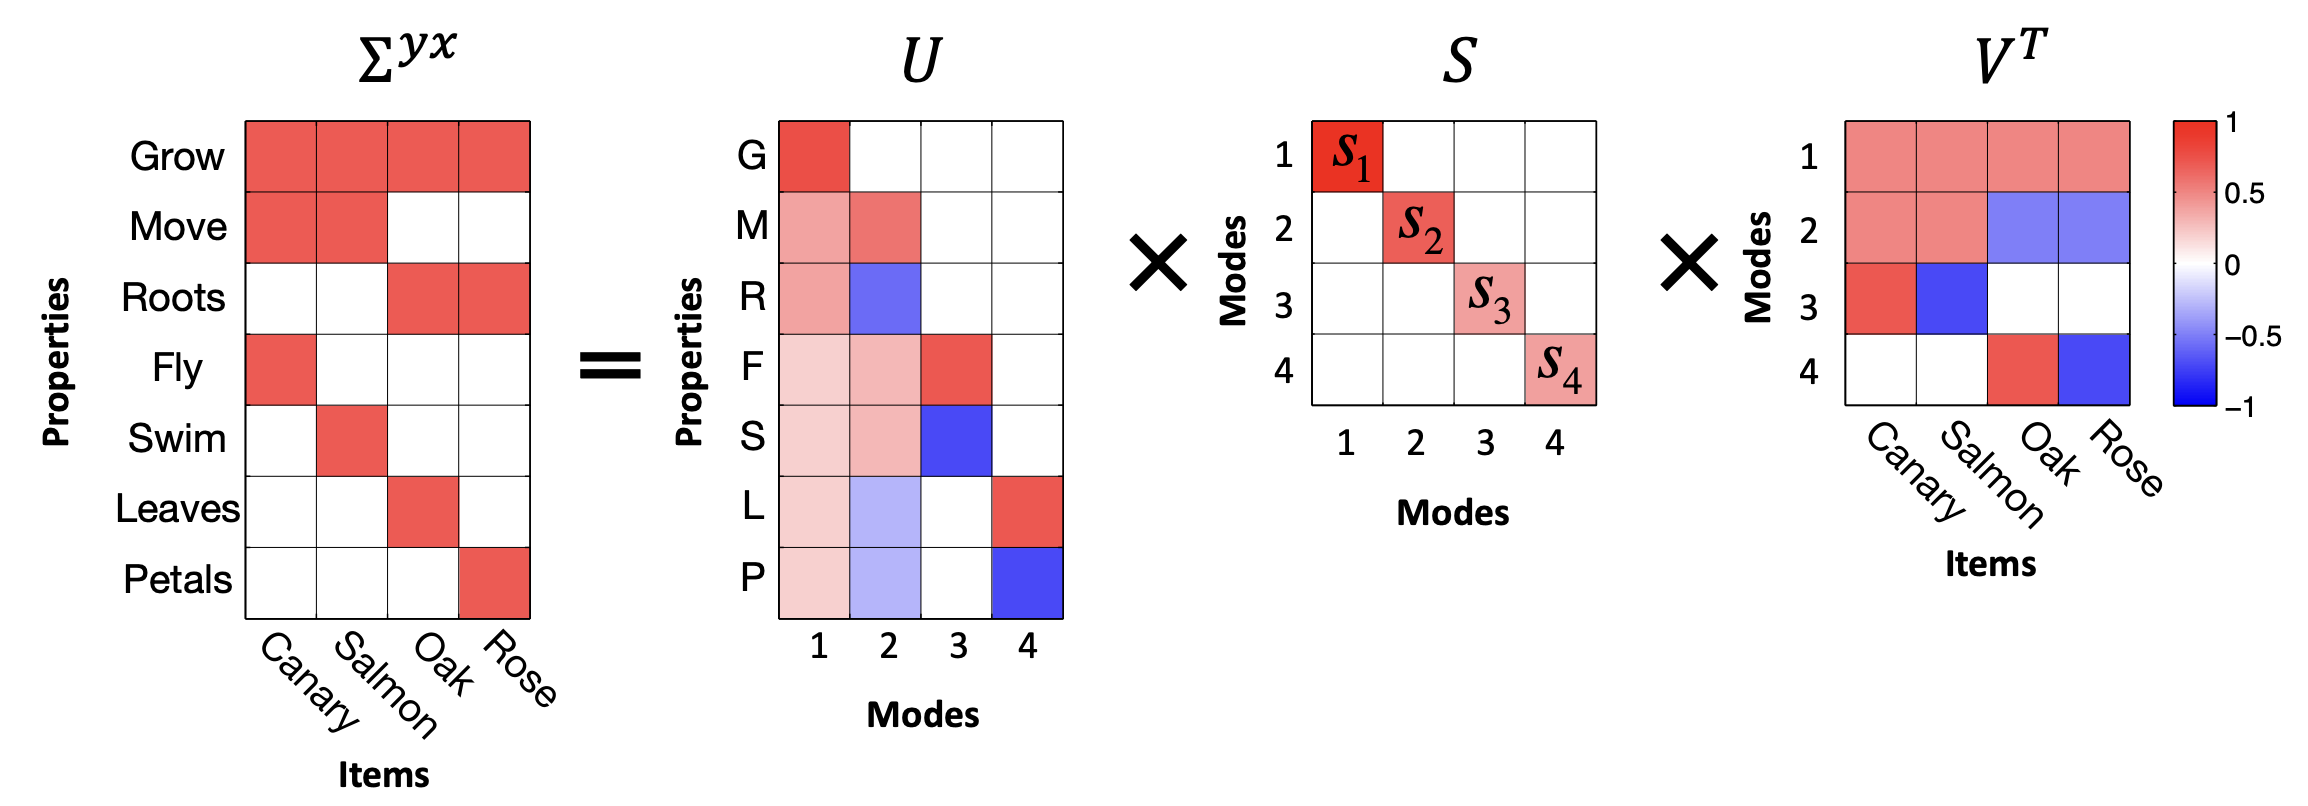
\includegraphics[width=0.8\linewidth]{figures/ch2-svd.png}
    \caption{Modes link a set of coherently covarying properties with a set of
    coherently covarying items.}
    \label{fig:ch2-svd}
\end{figure}

Now we can give the SVD's two sets of axes a tangible meaning.

The columns of $V^\star$ (equivalently, the rows of ${V^\star}^\top$) are the
\textbf{input modes}, or input-analyzing vectors. Each one places every input
item along a single interpretable semantic axis. The second input mode, for
instance, behaves like an ``animal--plant'' axis: animals like Canary and Salmon
land on the positive side, plants like Oak and Rose on the negative side. A single
direction in the input space has captured a coherent semantic distinction.

The columns of $U^\star$ are the \textbf{output modes}, or output-analyzing
vectors. Symmetrically, each one places every output \emph{feature} along a
semantic axis. Every input mode is paired with exactly one output mode, and the
singular value $\lambda^\star_\mu$ joining them measures that axis's
``categorizing power''---how much of the data's structure this one input-output
distinction accounts for. Big singular values are the broad, important cuts
through the data (animal vs.\ plant); small ones are the subtle, subordinate
details (which specific kind of bird).

The thing to take away---and the reason this example is worth dwelling on---is that
the SVD isn't just an algebraic convenience we reached for to make an integral
tractable. It is carving the data up along genuinely meaningful semantic
directions, and those very directions, as we're about to see, are the directions
the network learns \emph{one at a time, in order of importance}.

\subsection{Step 3: Argue that weight alignment happens quickly}

Our diagonalized equations of motion are cleaner than before, but they're still
coupled: $\tilde{W}_1$ and $\tilde{W}_2$ both appear inside each other's updates,
so we can't yet solve for either one on its own. The entire goal of this step is
to find a condition under which the coupling falls apart---under which the
dynamics \emph{decouple} into a bunch of independent one-dimensional problems we
can integrate by hand.

We're going to proceed by identifying a special condition (we'll call it \emph{weight alignment}) that, if true, makes everything decouple. Then we're going to argue---somewhat informally---that small initialization makes
this condition come true very quickly, early in training. We will \emph{not} prove
this rigorously. Instead we'll do something that is, in its own way, just as convincing, and we'll come back to it at the end of the next step.

\subsubsection*{What condition would decouple the dynamics?}

To find the condition we want, it helps to keep thinking spectrally---that is, in
terms of the SVD. Recall that the SVD splits any matrix into \emph{directions}
(the singular vectors, $U$ and $V$) and \emph{magnitudes} (the singular values,
$S$). The coupling in our equations lives entirely in the \emph{directions}. If the directional parts of the two weight matrices were
already settled and pointing the right way, the only thing left to evolve would be
the magnitudes---and magnitudes are just numbers, which decouple easily.

So let's write each weight matrix in its SVD form, $W_1 = U_1 S_1 V_1^\top$ and
$W_2 = U_2 S_2 V_2^\top$, and ask: under what directional conditions does the
model $\tilde{W}_2 \tilde{W}_1$ collapse to a clean product of magnitudes,
$S_2 S_1$, with all the rotation matrices canceling out? Working it
through,\footnote{To see it, write the rotated model in terms of the weight SVDs:
$\tilde{W}_2 \tilde{W}_1 = (U^{\star\top} W_2)(W_1 V^\star) = U^{\star\top}U_2\,
S_2\, V_2^\top U_1\, S_1\, V_1^\top V^\star$. Now impose the three conditions:
$U_2 = U^\star$ makes $U^{\star\top}U_2 = I$; $V_2 = U_1$ makes $V_2^\top U_1 = I$;
and $V_1 = V^\star$ makes $V_1^\top V^\star = I$. All the rotation matrices
collapse to identities and we're left with $\tilde{W}_2 \tilde{W}_1 = S_2 S_1$, a
product of pure magnitudes.} you need three things to line up:
\begin{enumerate}
    \item $U_2 = U^\star$ --- the output directions of $W_2$ match the data's
    output modes.
    \item $V_1 = V^\star$ --- the input directions of $W_1$ match the data's input
    modes.
    \item $V_2 = U_1$ --- the directions where $W_1$ ``hands off'' to $W_2$ match
    each other.
\end{enumerate}

We'll call these three conditions together \textbf{weight alignment}. Conditions 1
and 2 say the network is aligned with the \emph{data} (its ends point along the
data's modes); condition 3 says the two layers are aligned with \emph{each other}
(they interface cleanly, with no rotational mismatch in the middle). When all
three hold, only the singular values along the diagonals of $S_1$ and $S_2$ are left to evolve, and---as we'll confirm in Step 4---those evolve independently, mode by mode. That's the
decoupling we're after.

\subsubsection*{Why small initialization gets us there}

These three conditions are demanding, and there's no reason a randomly initialized
network should satisfy them. So why should we expect alignment to happen at all?

The answer is that it reliably happens, fast, in one specific setting: the
\textbf{small initialization regime}, where we start all the weights very close to
zero so that they have to \emph{grow} substantially over training. This is in
contrast to the \emph{large initialization} or ``lazy'' regime, where weights
start big and barely move from their random starting point---in which case no
interesting directional structure ever develops, and none of the phenomena in
this chapter appear. We'll have more to say about that contrast later. Small
initialization forces alignment through two separate mechanisms, one for the
layers-with-each-other condition and one for the layers-with-data conditions.

We'll sketch both. Feel free to skim these---the precise arguments lean on a bit
of perturbation theory and on power iteration, and the original
\href{https://arxiv.org/pdf/1312.6120}{Saxe et al.\ (2013)} derivation simply
\emph{assumed} fast alignment without proving it. The takeaway you actually need
is just that \emph{from small initialization, alignment happens quickly.}

\paragraph{Inner alignment (the layers align with each other), via the
conservation law.} Here we get to spend the conservation law we banked in Step 1.
Recall $H := W_2^\top W_2 - W_1 W_1^\top$ is conserved for all time. From small
initialization, the weights start tiny, so $H$ starts tiny---and because it's
conserved, it \emph{stays} tiny even after the weights have grown large. That
means that once training is underway,
\begin{align*}
    W_2(t)^\top W_2(t) = W_1(t) W_1(t)^\top + \text{(a tiny perturbation)}.
\end{align*}
This near-equality of the two layers' Gram matrices is what we earlier named
\textbf{balancedness} ($H \approx 0$). And balancedness is enough to pin the
layers' directions together, by way of a classical result called the
\textbf{Davis--Kahan $\sin\theta$ theorem}. In plain terms, that theorem says: if
two symmetric matrices differ only by a small amount, \emph{and} their own
eigenvalues are well separated from each other, then they must share essentially
the same eigenvectors. Here the two matrices are $W_1 W_1^\top$ and $W_2^\top W_2$,
they differ only by the tiny $H$, and small initialization makes their eigenvalue
gaps grow large compared to $\|H\|$---so the theorem applies and forces their
relevant directions to coincide. That's precisely condition 3, inner alignment
($V_2 = U_1$). (A companion fact, Weyl's inequality, similarly forces the two
layers' singular \emph{values} to agree---which we'll use in Step 4.)

\paragraph{Outer alignment (the layers align with the data), via power iteration.}
The conservation law explains why the two layers snap to each other, but not why
they snap to the \emph{data's} modes. For that, look again at the whitened
equation of motion at the very start of training:
\begin{align*}
    \frac{d}{dt}W_1 = W_2^\top(\Sigma_{yx} - W_2 W_1).
\end{align*}
At initialization the weights are minuscule, so $W_2 W_1 \ll \Sigma_{yx}$ and that
term is negligible. The update simplifies to
\begin{align*}
    \frac{d}{dt}W_1 \approx W_2^\top \Sigma_{yx}.
\end{align*}
Look at what this is doing: at each instant the weights are getting multiplied by
$\Sigma_{yx}$ again and again. Repeatedly multiplying a vector (or matrix) by a
fixed matrix is exactly \textbf{power iteration}, the standard algorithm for
extracting a matrix's \emph{dominant} direction---because the largest singular
value gets amplified the most with each multiplication, it quickly drowns out the
rest. So this early phase acts like power iteration on $\Sigma_{yx}$: it
aggressively rotates $W_1$'s top directions to point along $\Sigma_{yx}$'s top
directions ($V_1 \to V^\star$), which is conditions 1 and 2, outer alignment. By
the time the weights have grown enough that the $W_2 W_1$ term stops being
negligible, this rotation is already a done deal---the directions are locked, and
only magnitudes remain to evolve.

So both mechanisms point the same way: from small initialization, the network
rushes into alignment before it does much else. We'll \emph{assume} alignment
holds from here on. We'll empirically justify this assumption later on as well.

\subsection{Step 4: Decouple the dynamics and solve}

Now let's use the alignment assumption to actually solve for the learning curve.
The plan: impose alignment to kill the directional coupling, reduce the matrix
equations to a single scalar ODE per mode, and integrate that ODE in closed form.

With alignment assumed, our equations of motion involve only the (diagonal)
singular-value matrices:
\begin{align}
    \frac{d}{dt}S_1 &= S_2 (\Lambda^\star - S_2 S_1)\\
    \frac{d}{dt}S_2 &= (\Lambda^\star - S_2 S_1) S_1.
\end{align}

Every matrix here is diagonal. This has two happy consequences. First, it
confirms that alignment is \emph{self-sustaining}: there's no off-diagonal term
left to rotate anything, so once the weights are aligned, gradient flow keeps them
aligned forever---alignment is a fixed point of the directional dynamics, not a
fleeting coincidence. Second, because the matrices are diagonal, the diagonal
entries don't talk to each other at all. The single coupled matrix problem has
shattered into many \emph{independent scalar problems}, one per mode. This is the
decoupling we've been chasing since Step 3.

We can simplify one more notch. Back in Step 3, balancedness (via Weyl's
inequality) told us the two layers' singular values agree, $S_1 \approx S_2$
throughout training in the small-initialization regime. So we can drop the
subscripts and write a single $S(t) := S_1(t) \approx S_2(t)$. The full network's
end-to-end map then has singular values $S^2$---one factor of $S$ from each layer.
Focusing on a single mode $\mu$ and applying the chain rule to its end-to-end
singular value $s_\mu^2$:
\begin{align*}
    \frac{d}{dt}s_\mu^2 &= 2 s_\mu \frac{d}{dt}s_\mu \notag \\
    &= 2 s_\mu^2 (\lambda^\star_\mu - s_\mu^2).
\end{align*}

\emph{This} is something we can solve. It's a
separable ODE: all the $s_\mu^2$ terms go on one side, all the $t$ terms on the
other, and we integrate directly.\footnote{Carrying out this integration---separate
variables, expand $\frac{1}{s^2(\lambda^\star - s^2)}$ by partial fractions,
integrate both sides, and solve for $s^2_\mu(t)$---is a clean, self-contained
calculation that lands exactly on the boxed logistic. It's left as an exercise at
the end of the chapter.} Out comes
\begin{equation}
    \boxed{s^2_\mu(t) = \frac{\lambda^\star_\mu}{1 + \left(\dfrac{\lambda^\star_\mu}{s^2_\mu(0)} - 1\right) e^{-2 \lambda^\star_\mu t}}}
    \label{eq:solution}
\end{equation}

Take a breath and appreciate what just happened: we have an exact, closed-form
expression for the strength of every mode of the network at every moment of
training. We started with a coupled, nonlinear, matrix-valued dynamical system,
and through one symmetry-derived assumption we've reduced it to a relatively simple scalar formula.

And the formula has a shape that we can recognize. It's a \textbf{logistic} (sigmoid)
function of time: each mode's strength $s_\mu^2(t)$ sits patiently near its tiny
initial value $s^2_\mu(0)$ for a while, then rapidly rises, then saturates at its
target value $\lambda^\star_\mu$. Learning a mode is not a steady grind---it's a
sudden transition, a switch flipping from ``off'' to ``on.''

Assembling the modes back together, the picture of the whole network is this: a
fast initial alignment phase, after which the network keeps the \emph{same
directions} as the data ($\Sigma_{yx}$'s singular vectors) for the rest of
training, and only the \emph{magnitudes} change, each riding its own sigmoid:
\begin{align*}
    W_2(t) W_1(t) \approx U^\star S^2(t) {V^\star}^\top
    = \sum_\mu s^2_\mu(t)\; u_\mu v_\mu^\top.
\end{align*}

\subsubsection*{Does any of this actually happen? Let's check.}

Recall that we made an assumption which we technically didn't
prove---that alignment happens quickly from small initialization---and used it to make a clean prediction, the boxed sigmoid above. That prediction is
\emph{testable}. We can train an actual 2-layer linear network from small random
weights, watch the strength of each mode evolve, and overlay our formula on top of
the measured curves. If our unproven assumption were badly wrong, the prediction
would miss, and we'd know it.

It doesn't miss. The analytical sigmoids (red) sit right on top of the measured
dynamics of the real network (blue).

\begin{figure}[H]
    \centering
    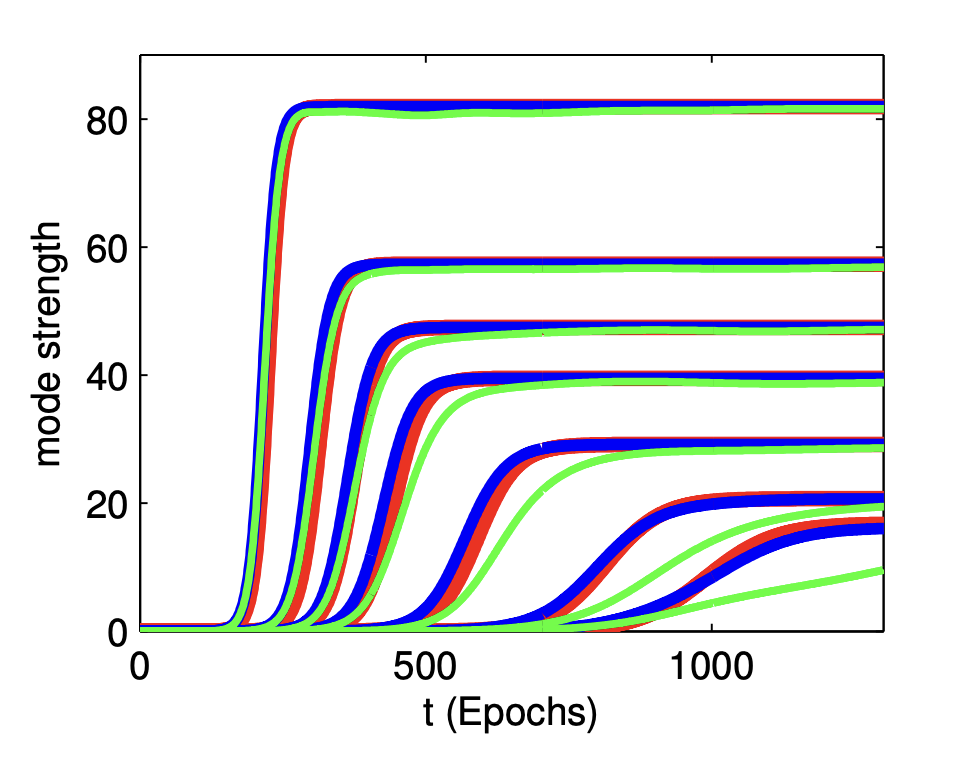
\includegraphics[width=0.4\linewidth]{figures/ch2-svcurves.png}
    \caption{Dynamics of learning in a 2-layer linear network. Curves show the
    strength of the network's representation of seven modes of the input-output
    correlation matrix over the course of learning. Red traces show our analytical
    sigmoids. Blue traces show simulation of the full dynamics of a 2-layer linear
    network from small random initial conditions. Green traces show simulation of
    a \emph{nonlinear} 2-layer network with tanh activation functions.}
    \label{fig:svcurves}
\end{figure}

This illustrates one of the most important tools
in a learning mechanic's toolkit. We rarely get to
prove everything rigorously; the systems are too tangled for that. So instead we
do this: \emph{make a reasonable-looking assumption, derive a theory from it, and
squeeze that theory for concrete, checkable predictions.} Then we go to the
empirics. If the predictions come out tight against reality---as they do here---that
agreement is itself strong evidence, working backward, that the theory is sound
and that the assumption we leaned on was in fact reasonable. A theory that makes sharp predictions and keeps getting them right is a theory
worth trusting.

\section{Saddle-to-saddle training dynamics}

We now have, in the boxed sigmoid from the last section, a complete description of
\emph{how} each mode is learned. The natural next questio is \emph{when}.
If every mode follows its own sigmoid, and each sigmoid switches on at its own
time, then the order and spacing of those switch-on times is the whole story of
the training curve. Let's compute it.

A clean way to summarize ``when is mode $\mu$ learned'' is to ask for its
\textbf{halfway-time} $\tau_\mu$: the moment at which the mode reaches half its
final strength, $s^2_\mu(\tau_\mu) = \tfrac{1}{2}\lambda^\star_\mu$. Setting the
sigmoid equal to $\tfrac12\lambda^\star_\mu$ and solving for $t$ (and dropping
order-one constants, which don't affect the qualitative story) gives a strikingly
simple scaling:\footnote{Filling in this short calculation is left as an exercise
at the end of the chapter.}
\begin{equation}
    \tau_\mu \approx \frac{1}{\lambda^\star_\mu} \ln \frac{\lambda^\star_\mu}{s^2_\mu(0)}.
\end{equation}

Read this formula and a clear prediction jumps out. The learning time is inversely
proportional to the mode strength $\lambda^\star_\mu$: \textbf{big modes are
learned first, small modes last.} And we know from the Canary example what that
means semantically---big modes are the coarse, dominant distinctions in the data
(animal vs.\ plant), small modes the fine subordinate details. So the network
learns the broad strokes of its task before the fine print, and it does so in a
strict, predictable order set entirely by the data's singular values. This is the
precise, quantitative version of the first piece of folklore we opened the chapter
with.

Now look at the \emph{spacing} between consecutive switch-on times, $\tau_\mu$ and
$\tau_{\mu+1}$. Notice the initialization scale $s^2_\mu(0)$ sits inside a
logarithm in the formula: as we shrink the initialization, every $\tau_\mu$ grows,
but they grow by different amounts, and the gaps between them stretch out. The
smaller the initialization, the more cleanly separated in time the modes
become---the sigmoids stop overlapping and instead fire one after another, in
distinct stages.

This is exactly what we see when we plot the loss: a \textbf{staircase loss curve.} Training from small
initialization, the loss doesn't fall smoothly. It sits on a long flat
\emph{plateau}, then drops sharply, then plateaus again, then drops. Our theory tells us precisely what each part of the staircase is: a
plateau is a stretch of time when no mode is transitioning (every sigmoid is
either still off or already saturated), and a sudden drop is the instant a new
mode switches on and the network suddenly captures a new chunk of the data's
structure.

\begin{figure}[H]
    \centering
    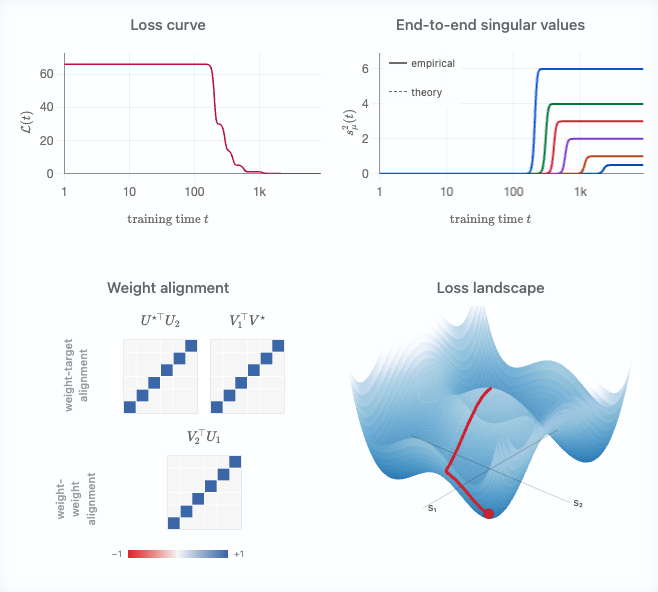
\includegraphics[width=0.65\linewidth]{figures/ch2-saddle.png}
    \caption{As initialization shrinks, the mode sigmoids separate in time and the
    loss curve develops distinct plateaus and drops---the staircase.}
    \label{fig:saddle}
\end{figure}

\subsection{Why the staircase? A landscape full of saddles}

The right way to understand the staircase loss curve is to picture the geometry of the loss landscape.
First we'll show
that the origin---where we start, under small initialization---is a saddle point.
Then we'll see how each mode contributes its own saddle, so that the full
landscape is riddled with them. Finally we'll watch a ball released near the
origin thread its way through this landscape, and the staircase will fall right
out.

\subsubsection*{The origin is a saddle}

Let's zoom all the way in to the simplest possible case---a single mode, with
everything reduced to scalars. The two weights $w_1$ and $w_2$ are just numbers,
the target is a positive number $\lambda^\star$, and the loss is
\begin{align*}
    \Lcal(w_1, w_2) = \tfrac{1}{2}(\lambda^\star - w_1 w_2)^2.
\end{align*}

What does this landscape look like right at the origin, $w_1 = w_2 = 0$? Take the
gradient and you'll find it's exactly zero there: the origin is a flat, stationary
point, a place where the ball, once placed, feels no pull. But ``stationary''
doesn't tell us its shape. Is it the bottom of a bowl (a minimum), the top of a
hill (a maximum), or something else? The way to find out is to stand at the origin
and take a small step in a couple of directions and see which way the ground
tilts.

Step along the direction where $w_1 = w_2$. Their product $w_1 w_2$ becomes
positive, which nudges the prediction $w_1 w_2$ \emph{toward} the target
$\lambda^\star$, so the loss goes \textbf{down}---you're walking downhill.

Now step along the direction where $w_1 = -w_2$. Their product becomes negative,
dragging the prediction \emph{away} from the positive target $\lambda^\star$, so
the loss goes \textbf{up}---you're walking uphill.

A stationary point with a downhill direction \emph{and} an uphill direction is
exactly what we mean by a \textbf{saddle point}; kinda like the surface of a Pringle. The origin is a saddle.

\subsubsection*{One saddle per mode, and a combinatorial explosion of
them}

Now zoom back out to the full, multi-dimensional network. Because the SVD decoupled the dynamics into independent
modes, the total loss is essentially just a \emph{sum} of independent single-mode
losses (this holds in the
aligned, decoupled regime we established in Step 4):
\begin{align*}
    \Lcal \approx \sum_{\mu} \tfrac{1}{2}(\lambda^\star_\mu - s_\mu^2)^2.
\end{align*}

When is the whole network stationary---when do \emph{all} the gradients vanish at
once? Looking at the sum, every mode has to be individually stationary, and we
just learned that each mode is stationary in exactly two situations: either it has
been \emph{perfectly learned} ($s_\mu^2 = \lambda^\star_\mu$, the bottom of that
mode's valley) or it has been \emph{completely ignored} ($s_\mu = 0$, that mode's
saddle at the origin).

Two possibilities per mode, chosen independently, means that if the data has $k$
modes, the landscape has $2^k$ stationary points (within this decoupled mode
picture). That's a lot of places for a ball to get stuck. Let's sort them:
\begin{itemize}
    \item Exactly \textbf{one} is the global minimum---every mode learned,
    $s_\mu^2 = \lambda^\star_\mu$ for all $\mu$. This is the answer we want.
    \item Exactly \textbf{one} is the master saddle at the origin---every mode
    ignored. It's the \emph{highest-loss} of all the critical points (nothing has
    been learned yet), and it's a saddle, because, as we saw in Movement 1,
    stepping away from it along any mode's downhill direction lowers the loss.
    \item \textbf{Every one of the other $2^k - 2$ stationary points is also a
    saddle.} Suppose the largest mode is fully learned
    ($s_1^2 = \lambda^\star_1$) but the second mode is still untouched
    ($s_2 = 0$). Along the first mode's coordinate, the network is sitting
    comfortably at the bottom of a valley. But along the second mode's
    coordinate, it is sitting \emph{exactly on that mode's origin-saddle}, with an
    unexploited downhill direction right there. A point that is a valley-bottom in
    some directions and a saddle in others is, overall, still a saddle. So this
    ``first mode learned, rest ignored'' state is at an
    unstable equilibrium.
\end{itemize}

\subsubsection*{The kinematics of escaping a saddle}

When we initialize with
very small random weights, we are setting the ball down a hair's breadth from the
master saddle at the origin. It starts to roll---but because the weights are tiny,
the gradients are tiny too, and it rolls \emph{excruciatingly} slowly. This is the
source of the very first plateau.

Which way does it go? Recall from Movement 1 that each mode's downhill steepness is
governed by its singular value $\lambda^\star_\mu$---and in fact, near the origin,
each mode's strength grows exponentially at a rate set by $\lambda^\star_\mu$
(this is the power-iteration effect from Step 3). So the ball accelerates down the direction
of the \emph{largest} mode exponentially faster than any other, slides down the
$s_1$ axis, and escapes the master saddle along that one direction.

Then it arrives at the next saddle: $(s_1^2 = \lambda^\star_1,\ s_2 = 0,\ s_3 = 0,
\dots)$---first mode learned, rest still at zero, an unstable equilibrium. Because the gradients for every \emph{remaining}
mode are still microscopically small, the ball slows down and the loss plateaus. But it hasn't stopped. Beneath the surface, $s_2$ is quietly growing,
exponentially, driven by the same power-iteration pull. Eventually it grows large
enough to tip the ball over the edge of \emph{this} saddle, and the ball slides
rapidly down the $s_2$ axis---which we see, up at the level of the loss curve, as a
sudden steep drop. It settles onto the next ledge, and the waiting game begins
again for mode 3. Plateau, drop, plateau, drop. This shows up as a staircase loss curve.

It's remarkable that in this toy example, we're able to make a concrete 
connection between what the network is learning and what the optimization dynamics look like. 
This can be thought of as an instantiation of the learning mechanics idea that learning, at its core,
is movement through high dimensional space.

\subsection{Saddle-to-saddle as implicit regularization}

Notice that because modes are learned in strict order of importance, a
network that we stop \emph{partway} through training will have captured only the
top few modes of $\Sigma_{yx}$, leaving all the rest still pinned near zero. In
other words, gradient descent from small initialization has a built-in preference
for \emph{simple, low-rank solutions}, adding complexity one mode at a time and
only as training proceeds. This is \textbf{implicit regularization} again---the
very phenomenon we met in Chapter 1, where gradient descent on linear regression
quietly preferred the minimum-norm solution without being told to. There, the bias
was toward small norm; here, it's toward low rank. In both cases, gradient descent
is doing something we never explicitly asked it to, biasing itself toward
simplicity.

\section{So what have we learned from all this?}

We started with four pieces of deep learning folklore that seemed like clues to deeper understanding which we wanted to capture in a toy model:
\begin{enumerate}
    \item deep learning learns the components of its target function in a
    preferred order;
    \item deep learning optimizes just fine, despite a wickedly nonconvex loss
    landscape;
    \item instantaneous training dynamics are often low-rank within each weight
    matrix; and
    \item we tend to get stepwise, staircase loss curves, especially when training
    from small initialization.
\end{enumerate}

Deep linear nets capture all of these. So, what now? Did all this reveal any deeper insight into the fundamental reasons for these folklore observations?

By and large, yes! We can revisit each of these four folklore beliefs with a new perspective.

\paragraph{1. The preferred learning order.} We can now say exactly what sets it:
the data, through its covariances. The order depends on the input statistics
($\Sigma_{xx}$) and the target relationship ($\Sigma_{yx}$) together, and the rule
is that larger components of the target along larger directions of the input are
learned faster---precisely our $\tau_\mu \propto 1/\lambda^\star_\mu$ result.
Reassuringly, real \emph{nonlinear} networks share this same bias toward quickly
learning functions of the data's large directions which
is a sign our linear toy model caught something real rather than an artifact of
linearity.

\paragraph{2. Optimizing a nonconvex landscape.} We saw that the fearsome
nonconvex landscape of a deep linear network actually decomposes, after alignment,
into many simple one-dimensional subproblems solved in parallel---one per mode.
This decomposition won't hold exactly for nonlinear networks. But it makes the
folklore far less mysterious, and it dovetails with another widely held belief:
that large models are full of semi-independent ``circuits'' that can be understood
and optimized more or less separately. A landscape that looks hopeless globally
can be benign once you find the right pieces to look at.

\paragraph{3. Low-rank instantaneous dynamics.} In our model, the reason is now
transparent: at any given moment, typically just one singular value (or a few) is
in its rapid-growth phase, while the rest sit still. Each time a singular value
switches on, it opens up a new pathway from input to output---it \emph{looks like
a new circuit suddenly forming.} It’s possible that deep nonlinear networks show low-rank behavior for the similar reason that only a relatively small number of “circuits” are undergoing rapid development at a particular time. Of course, this is highly speculative and this explanation should be handled with care until tested.

\paragraph{4. Staircase loss curves.} This one we explained in full: the
parameters slide down a sequence of saddle points of decreasing order on their way
to a minimum, and the plateaus and drops are the lingering-and-descending of those
saddle-to-saddle dynamics. The same essential mechanism is believed to drive the
staircase curves seen in real nonlinear networks, and deep linear networks are now
the standard, well-understood toy model for the phenomenon.

\bigskip

So the toy model delivered: four behaviors, one solvable system. But let's be
honest about its limits, in the same spirit we were honest about linear regression
at the end of Chapter 1. A deep linear network, no matter how deep, can only ever
represent a \emph{linear} function of its input. Every phenomenon that
fundamentally requires learning a \emph{nonlinear} function of the data lies
completely outside its reach. And that, frustratingly, is \emph{most} of what we
ultimately want to understand about deep learning.

Still---and I hope this is the feeling you're left with---it's remarkable how far
one well-chosen simplification carried us. We kept depth and coupling, gave up the
nonlinearity, and in return got an exact, predictive, empirically validated
account of preferential learning, benign optimization, low-rank dynamics, and
staircase losses. Deep linear networks are the textbook example of a toy model
that is \emph{simple, but not too simple}: simple enough to solve with the tools in
hand, rich enough to teach us something true about the real thing.
\section*{Chapter 2 Exercises}

These exercises fill in the calculations we deferred in the main text. None of
them require any tools beyond what's in the chapter.

% ---------------------------------------------------------------------
\subsection*{2.1 The loss in covariance form.}
In the setup, we claimed that ``with some matrix algebra'' the mean squared error
can be rewritten purely in terms of the data covariances. Verify this. Starting
from
\begin{align*}
    \Lcal(W_1, \dots, W_L)
    = \mathbb{E}_{(x,y)\sim\Dcal}
      \Big[\Tr\,(y - W_L \cdots W_1 x)(y - W_L \cdots W_1 x)^\top \Big],
\end{align*}
expand the product inside the trace, use linearity of the trace and the
expectation, and substitute the definitions $\Sigma_{xx} := \mathbb{E}_\Dcal[xx^\top]$,
$\Sigma_{yx} := \mathbb{E}_\Dcal[yx^\top]$, and $\Sigma_{yy} := \mathbb{E}_\Dcal[yy^\top]$
to arrive at
\begin{align*}
    \Lcal(W_1, \dots, W_L)
    = \|\Sigma_{yx}\Sigma_{xx}^{-1/2} - W_L \cdots W_1 \Sigma_{xx}^{1/2}\|_\mathrm{F}^2
      + \mathrm{const.}
\end{align*}
where $\mathrm{const.} = \Sigma_{yy} - \Sigma_{yx}(\Sigma_{xx})^{-1}(\Sigma_{yx})^\top$.
Confirm that the constant term does not depend on the weight matrices.

\emph{Hint:} ``complete the square'' at the level of matrices---add and subtract
$\Sigma_{yx}\Sigma_{xx}^{-1/2}$ inside the Frobenius norm.

% ---------------------------------------------------------------------
% \begin{exercise}[The conservation law, by the algebra trick.]
% Derive the conservation law of Equation~(\ref{eq:conservation-ex}) the same way the
% chapter body does.
% \begin{enumerate}[label=(\alph*)]
%     \item Compute the gradients $\nabla_{W_1}\Lcal$ and $\nabla_{W_2}\Lcal$ for the
%     2-layer loss and confirm the gradient flow equations
%     \begin{align*}
%         \frac{d}{dt}W_1 &= W_2^\top(\Sigma_{yx} - W_2 W_1 \Sigma_{xx}), &
%         \frac{d}{dt}W_2 &= (\Sigma_{yx} - W_2 W_1 \Sigma_{xx}) W_1^\top.
%     \end{align*}
%     \item Using these, show that
%     $\big(\tfrac{d}{dt}W_1\big)W_1^\top = W_2^\top\big(\tfrac{d}{dt}W_2\big)$, and
%     hence that
%     \begin{equation}
%         \frac{d}{dt}\big(W_2^\top W_2 - W_1 W_1^\top\big) = 0.
%         \label{eq:conservation-ex}
%     \end{equation}
%     \item Conclude that $H := W_2^\top W_2 - W_1 W_1^\top$ is constant along the
%     gradient flow trajectory, so a network initialized balanced ($H \approx 0$)
%     stays balanced.
% \end{enumerate}
% \end{exercise}

% ---------------------------------------------------------------------
\subsection*{2.2 The conservation law, from the symmetry.}
The algebra trick used in the chapter to derive the conservation law $\frac{d}{dt}[W_2^\top W_2 - W_1 W_1^\top] = 0$ derives it as if by
luck. This exercise re-derives it from the continuous
symmetry of the loss, making clear \emph{why} the trick works.

Throughout, use the matrix inner product $\langle A, B\rangle := \Tr(A^\top B)$,
and recall the gradient flow $\dot\theta = -\nabla\Lcal$ for $\theta = (W_1, W_2)$.

\begin{enumerate}[label=(\alph*)]
    \item \emph{(Symmetry $\Rightarrow$ orthogonality.)} Suppose $\Lcal$ is
    invariant under a one-parameter family of transformations
    $\theta \mapsto \theta + \epsilon\, v(\theta)$, with generator (velocity field)
    $v$. Show that invariance, to first order in $\epsilon$, is equivalent to
    \begin{align*}
        \langle v(\theta), \nabla\Lcal(\theta)\rangle = 0 \quad \text{for all } \theta.
    \end{align*}
    \item \emph{(Gradient flow never moves along the symmetry.)} Substitute the
    gradient flow equation to conclude that $\langle v(\theta), \dot\theta\rangle = 0$
    along any trajectory. Interpret this geometrically: the gradient flow velocity
    is always orthogonal to the symmetry direction, so optimization never spends
    motion traveling along the symmetry orbit.
    \item \emph{(The specific symmetry.)} For the deep linear network, the symmetry
    is $W_1 \mapsto AW_1,\ W_2 \mapsto W_2 A^{-1}$. Take $A = e^{\epsilon M} \approx
    I + \epsilon M$ for an arbitrary generator matrix $M$, and show that the
    induced generator is $v = (M W_1,\ -W_2 M)$.
    \item \emph{(All generators at once.)} Plug this $v$ into the orthogonality
    condition from (b), substitute $\nabla_{W_1}\Lcal = -\dot W_1$ and
    $\nabla_{W_2}\Lcal = -\dot W_2$, and use the cyclic property of the trace to
    rewrite both terms with $M^\top$ pulled to the front. Show the condition
    becomes
    \begin{align*}
        \Tr\!\big(M^\top \dot W_1 W_1^\top\big) = \Tr\!\big(M^\top W_2^\top \dot W_2\big).
    \end{align*}
    \item \emph{(Conclude.)} Since this must hold for \emph{every} generator $M$,
    deduce that $\dot W_1 W_1^\top = W_2^\top \dot W_2$, which is exactly
    $\frac{d}{dt}(W_2^\top W_2 - W_1 W_1^\top) = 0$. Note where the arbitrariness of
    $M$ was essential: it is what upgrades a single scalar orthogonality condition
    into the full matrix-valued conservation law.
\end{enumerate}

\emph{Remark.} Compare this derivation to the algebra trick. The trick yields
$\dot W_1 W_1^\top = W_2^\top \dot W_2$ by a fortunate cancellation; here the
\emph{same} equation appears as the direct consequence of ``the flow is orthogonal
to every symmetry direction.'' The luck of the trick was the symmetry in disguise
all along.

% ---------------------------------------------------------------------
\subsection*{2.3 Alignment collapses the model to its magnitudes.}
Write the weight SVDs as $W_1 = U_1 S_1 V_1^\top$ and $W_2 = U_2 S_2 V_2^\top$, and
recall the rotated model $\tilde{W}_2 \tilde{W}_1 = U^{\star\top} W_2 W_1 V^\star$,
where $\Sigma_{yx} = U^\star \Lambda^\star {V^\star}^\top$. Show that under the
three weight-alignment conditions,
\begin{align*}
    U_2 = U^\star, \qquad V_1 = V^\star, \qquad V_2 = U_1,
\end{align*}
the rotated model reduces to the product of magnitude matrices,
$\tilde{W}_2 \tilde{W}_1 = S_2 S_1$, with all rotation factors canceling. Identify
which orthogonality relation kills each rotation factor.

% ---------------------------------------------------------------------
\subsection*{2.4 Solving the scalar learning dynamics.}
This is the climactic integration of the chapter. The $\mu$-th end-to-end singular
value obeys the separable ODE
\begin{align*}
    \frac{d}{dt}s_\mu^2 = 2 s_\mu^2 (\lambda^\star_\mu - s_\mu^2).
\end{align*}
Let $u := s_\mu^2$ for brevity, so that $\dot{u} = 2u(\lambda^\star_\mu - u)$.
\begin{enumerate}[label=(\alph*)]
    \item Separate variables and use the partial-fraction identity
    \begin{align*}
        \frac{1}{u(\lambda^\star_\mu - u)}
        = \frac{1}{\lambda^\star_\mu}\left(\frac{1}{u} + \frac{1}{\lambda^\star_\mu - u}\right)
    \end{align*}
    to integrate both sides from $0$ to $t$.
    \item Solve the resulting expression for $u = s_\mu^2(t)$ and confirm you
    recover the logistic solution
    \begin{align*}
        s^2_\mu(t) = \frac{\lambda^\star_\mu}
        {1 + \left(\dfrac{\lambda^\star_\mu}{s^2_\mu(0)} - 1\right) e^{-2 \lambda^\star_\mu t}}.
    \end{align*}
    \item Check the two limits: confirm that $s_\mu^2(t) \to s_\mu^2(0)$ as
    $t \to 0$ and $s_\mu^2(t) \to \lambda^\star_\mu$ as $t \to \infty$.
\end{enumerate}

% ---------------------------------------------------------------------
\subsection*{2.5 Time-to-learn.}
Using the logistic solution from the previous exercise, derive the halfway-time
$\tau_\mu$ at which mode $\mu$ reaches half its final strength,
$s^2_\mu(\tau_\mu) = \tfrac{1}{2}\lambda^\star_\mu$. Show that, dropping order-one
constants,
\begin{align*}
    \tau_\mu \approx \frac{1}{\lambda^\star_\mu} \ln \frac{\lambda^\star_\mu}{s^2_\mu(0)}.
\end{align*}
Then argue from this expression that (a) larger modes are learned first, and (b)
the time-separation between consecutive modes widens as the initialization scale
$s^2_\mu(0)$ shrinks---the mechanism behind the cleanly separated stairsteps in
the loss curve.

\clearpage

\chapter{Toy Model II: Kernel Regression}
In the previous chapter we studied deep linear networks, i.e., networks that are a linear function of their input data. What made the analysis interesting was their nonlinear training dynamics. Such nonlinear training dynamics are a result of a subtlety in the word "\textit{linear}" in deep linear network. It's true that the network is linear with respect to each individual weight matrix $W_i$. However, if we consider the weights collectively, stacking all the scalar weights in one ginormous \textit{parameter vector} $\theta$, then a deep linear network is decidedly \textit{not} linear in $\theta$. In fact, a deep linear network with $L$ layers is an $L$th order polynomial of $\theta$. This is essentially what results in coupled dynamics and why we had to solve nonlinear ODEs to obtain the optimization trajectories of the weights. This is also what made deep linear networks a decent toy model of neural network training dynamics. 

In this chapter, instead of networks that are a linear function of their input data, we will study networks that are approximately a linear\footnote{Technically affine.} function of their parameter vector $\theta$. A good way to think about such networks is that their weights $\theta$ deviate so little from initialization throughout training that the network as a whole is well approximated by its first-order (linear) Taylor expansion centered at its weights at initialization $\theta^{(0)}$:

\begin{align}
    \hat{f}^{(t)}(x) &\approx \hat{f}^{(t)}_{\text{lin}}(t) := \hat{f}^{(0)}(x) + \left(\nabla_{\theta} \hat{f}(x) \rvert_{\theta=\theta^{(0)}}\right)^\top (\theta^{(t)}-\theta^{(0)}) \\
    &= \text{const.} + (\text{const. vector})^{\top}(\text{change in weights}) 
\end{align}

for all $t\geq0$. Crucially, the terms $\hat{f}^{(0)}(x)$ and $\nabla_{\theta} \hat{f}(x) \rvert_{\theta=\theta^{(0)}}$ are determined at initialization and stay constant throughout training. 
The weights of this kind of network undergo very simple, exactly solvable optimization trajectories. 
For neural networks in the infinite-width limit, 
there exist hyperparameter settings
that result in this kind of linear training.\footnote{There are also hyperparameter settings that result in non-lazy training in the infinite-width limit. More on that in the next chapter.}
Because the weights undergoing this kind of training barely move,
we say that such hyperparameter settings put the network in the \textit{lazy} regime.
It's also worth noting that a recent paper from Meterez et al. (2026)\footnote{A Defense of the Quadratic Model, https://arxiv.org/pdf/2607.21716} 
found that for LLMs, such a first-order Taylor expansion well-approximates the full model
for meaningful windows of time during pretraining.

\section{Lazy training in the infinite-width limit}

When dealing with coupled systems that have many moving parts, physicsts love to
take some parameter(s) to infinity and see if things simplify.
A classic example of this techinque is the thermodynamic limit. 
The key idea is that macroscopic behavior becomes stable and easier to analyze when
micro-level fluctuations vanish. Might something like that be possible for neural networks?


Consider a 2-layer neural network:

\begin{align}
\hat{f}(x) = W_2 \sigma(W_1 x).
\end{align}

We can rewrite this in a suggestable way as follows:

\begin{align}
\hat{f}(x) = \sum^H_{i=1}u_i \sigma(w^\top_i x)
\end{align}

where the $u_i\in\mathbb{R}^{n_\text{out}}$ are columns of $W_2\in\mathbb{R}^{{n_\text{out}}\times H}$ and the $w_i\in\mathbb{R}^{n_\text{in}}$ are rows of $W_1\in\mathbb{R}^{H\times{n_\text{in}}}$.
Written this way, it's clear that a 2-layer neural network is just an input-dependent linear combination
of output vectors $u_i$. Furthermore, at initialization, the pairs $(u_i, w_i)$ are drawn independently across $i$ from some fixed distribution. 
This means that for any fixed input $x$, the $H$ summands $u_i \sigma(w^\top_i x)=:X_i$
are themselves i.i.d.\ random vectors in $\mathbb{R}^\text{out}$. In other words,

\begin{align}
    \hat f(x) = \sum_{i=1}^H X_i
\end{align}

is precisely a sum of $H$ i.i.d. random vectors at initialization. 
This is exactly the kind of object the central limit theorem (CLT) governs. 

To cleanly make a CLT-style concentration argument, we need to send the number of summands to infinity, i.e., $H \to \infty$.
However, there's a problem with absent-mindedly taking this infinite-width limit: 
the value of the function $\hat{f}(x)$ will also go to infinity! 
One way to prevent $\hat{f}(x)$ from blowing up is to scale the output inversely proportional
to the size of the width $H$. 
Such output scaling allows us to initialize weights as 
standard Gaussians ($u_{ij}\sim\mathcal{N}(0,1)$ and $w_{ij}\sim\mathcal{N}(0,1)$)
and use a width-independent learning rate $\eta$.
By and large, there are two classical ways of scaling a sum of 
i.i.d. random variables:
a $\frac{1}{H}$ scaling and a $\frac{1}{\sqrt{H}}$ scaling.
The former is associated with the law of large numbers (LLN) while the latter is associated with
the central limit theorem (CLT). 
The latter is what leads to lazy training, so we'll study that first:

\begin{align}
\hat{f}^{(t)}(x) = \frac{1}{\sqrt{H}}\sum^H_{i=1}u^{(t)}_i \sigma({w^{(t)}}^\top_i x),
\label{ch3-clt-scaling}
\end{align}

where $u^{(0)}_{ij}\sim\mathcal{N}(0,1)$ and $w^{(0)}_{ij}\sim\mathcal{N}(0,1)$ and the learning rate $\eta$ is some small width-independent number (e.g., 0.1).
We'll see that this setup not only allows us to leverage the CLT at initialization,
it also results in the weights moving so little from initialization that 
for large $H$, the network $\hat{f}^{(t)}(x)$ is well-approximated by
its first-order Taylor expansion $\hat{f}^{(t)}_{\text{lin}}(x)$, i.e., it undergoes lazy training.

Concretely, we'll try to understand why the following statement
might be true:

\begin{align}
\sup_{t\geq 0} \left \| \hat{f}^{(t)}(x) - \hat{f}^{(t)}_{\text{lin}}(x) \right \|_2 = \mathcal{O}\left (\frac{1}{\sqrt{H}}\right ).
\end{align}

In the $H\to\infty$ limit, the above equation implies that
the trajectory of $\hat{f}^{(t)}(x)$ is exactly the trajectory of $\hat{f}^{(t)}_{\text{lin}}(x)$.
To make sense of the above statement, we will now introduce one of the central objects of study
in learning mechanics: the neural tangent kernel (NTK).

\subsection{The neural tangent kernel}

At its core, the neural tangent kernel is a tool for reasoning about 
networks undergoing gradient descent in \textit{function space} instead of \textit{weight space}.
Recall that weight space is the collection of all possible weight configurations.
It can be thought of as a high dimensional vector space $\mathbb{R}^M$ where
$M$ is the total number of tunable weights. Every point in this space of weights
is mapped to a scalar loss value by the loss function $\mathcal{L}:\mathbb{R}^M\to\mathbb{R}$.
These loss values make up the loss landscape.
In chapters 1 and 2, we mostly thought about networks' weight space dynamics; i.e.,
how the weights $\theta$ traverse the loss landscape according to gradient flow:

\begin{align}
\dot{\theta}^{(t)} = -\nabla_{\theta} \mathcal{L}(\theta^{(t)}).
\end{align}

However, at the end of the day, the only reason we care about the dynamics of
the weights $\theta$ is because they tell us about the dynamics of 
the network function $\hat{f}(x)$---we want to see how
the predictions for each data point $x\in\mathbb{R}^{n_{\text{in}}}$ evolve over time.
Could we bypass the middleman $\theta$\footnote{There are pros and cons to studying weight
space dynamics. On the one hand, it's the most visceral way to think about
what's going on during gradient descent. On the other hand, there's a lot of stuff
to keep track of and there exist many symmetries in weight space that create
annoying redundancies.}
 and directly
study the dynamics of the time-evolving prediction matrix
$\hat{f}^{(t)}(X)\in\mathbb{R}^{P\times n_{\text{out}}}$ 
(where $X\in\mathbb{R}^{P\times {n_{\text{in}}}}$
and $P$ is the number of data points in the training set)? 

For the rest of this chapter we take $n_\text{out}=1$ so that $\hat{f}(x)\in\mathbb{R}$ and
$\hat{f}(X)\in\mathbb{R}^P$\footnote{Nothing conceptual changes for $n_\text{out}>1$; the kernel
simply becomes an $Nn_\text{out}\times Nn_\text{out}$ matrix of blocks, one $n_\text{out}\times
n_\text{out}$ block per pair of training points.}. It will be convenient to name the Jacobian of the
network's predictions with respect to its weights,

\begin{align}
J^{(t)} := \frac{\partial \hat{f}^{(t)}(X)}{\partial \theta} \in\mathbb{R}^{P\times M},
\qquad
J^{(t)}_{ik} = \frac{\partial \hat{f}^{(t)}(x_i)}{\partial \theta_k},
\end{align}

whose $i$th row is the gradient of the network's prediction at $x_i$ with respect to all $M$
weights.

Now apply the chain rule to see how the predictions move:

\begin{align}
\dot{\hat{f}}^{(t)}(X)
= J^{(t)}\dot{\theta}^{(t)}
= - J^{(t)} \nabla_{\theta}\mathcal{L}
= - \underbrace{J^{(t)} {J^{(t)}}^{\top}}_{=:K^{(t)}}
\nabla_{\hat{f}(X)}\mathcal{L}\left(\hat{f}^{(t)}(X)\right),
\label{ch3-ntk-v2}
\end{align}

The matrix that
appeared is the \textit{empirical neural tangent kernel}:

\begin{align}
K^{(t)} := J^{(t)}{J^{(t)}}^\top \in\mathbb{R}^{P\times P},
\qquad
K^{(t)}_{ij} = \sum^M_{k=1} \frac{\partial \hat{f}^{(t)}(x_i)}{\partial \theta_k}
\frac{\partial \hat{f}^{(t)}(x_j)}{\partial \theta_k}.
\end{align}

For now, we'll refer to the empirical neural tangent kernel as simply the NTK.
The following are three important observations we can make about the NTK. 
First, $K^{(t)}$ is symmetric and positive semi-definite. 
Second, it has no information about the loss or the labels: it is built
entirely from the architecture and the current weights, and the loss enters
Equation~\eqref{ch3-ntk-v2} only through the separate factor $\nabla_{\hat{f}(X)}\mathcal{L}$. Third,
Equation~\eqref{ch3-ntk-v2} is exact. We have made no approximation, taken no limit, and assumed
nothing about the architecture; every neural network trained by gradient flow obeys it. Gradient
flow was used only to get a clean ODE, and the definition of $K^{(t)}$ itself is perfectly sound
under discrete gradient descent.

\subsubsection{Neural networks do a generalized version of linear regression}
\label{nn-lr}

Take a hard look at Equation~\eqref{ch3-ntk-v2}. Hopefully it looks familiar. It is almost exactly the
differential equation for overparameterized linear regression from chapter 1:

\begin{align}
\dot{\hat{f}}^{(t)}_{\text{linreg}}(X) = X\dot{w}^{(t)}
&= - X X^\top\left(Xw^{(t)}-y\right) \\
&= - X X^\top \nabla_{\hat{f}_{\text{linreg}}(X)}
\mathcal{L}\left(\hat{f}_{\text{linreg}}^{(t)}(X)\right).
\end{align}

Linear regression is the special case in which the Jacobian is the data matrix itself, $J = X$, so
that the kernel is just the matrix of inner products between data points,
$K_{ij} = x^\top_i x_j$. Being linear in its weights, linear regression has a Jacobian that does not
depend on $w$ at all, which is precisely why its kernel is constant and its dynamics are solvable in
closed form.

Define the \textit{feature map}

\begin{align}
\phi^{(t)}(x) := \frac{\partial \hat{f}^{(t)}(x)}{\partial \theta} \in \mathbb{R}^M,
\qquad\text{so that}\qquad
K^{(t)}_{ij} = \left\langle \phi^{(t)}(x_i), \phi^{(t)}(x_j)\right\rangle.
\end{align}

We can think of the NTK as first projecting each data point into an $M$-dimensional feature space, then taking inner
products there. Thus, a neural network can be thought of as doing linear regression in some high-dimensional
feature space using a data-dependent, time-evolving feature map $\phi^{(t)}$!
This is a powerful way to think about feature learning.

At this point, it might seem like we've cracked neural networks: 
they're just a more data-dependent version of linear regression.\footnote{
    In this sense, I lied a little when I said that linear regression is a terrible toy model
    of neural networks in chapter 1.
} A full understanding feels within reach. But this is an illusion.
All we've really done is push the problem of feature learning up one level of abstraction; 
from evolving weights to an evolving kernel. Studying the latter is not necessarily any easier than studying 
the former. That being said, the NTK isn't a dead end. 
It gives us a natural place to start: the lazy regime, where the kernel stays (approximately) 
frozen and the dynamics become tractable (essentially the same dynamics as linear regression).
Furthermore, we'll find that there are interesting insights to be gained about generalization
from networks in the lazy regime.

For a network that is linear in its weights, such as the linearization $\hat{f}_{\text{lin}}$ from
the start of this chapter, the NTK will stay constant throughout training. By construction
$\phi^{(t)}_{\text{lin}}(x) = \nabla_{\theta}\hat{f}(x)\rvert_{\theta=\theta^{(0)}}$ is independent
of $t$, so $K_{\text{lin}}^{(t)} = K^{(0)}$ exactly, for all $t$. 
Conversely, a fixed NTK implies that the network equals its linearization throughout training.
The dynamics of the linearized network are exactly those of a classical, well-studied statistical method:
\textit{kernel regression}. And we can solve it exactly like how we solved overparameterized 
linear regression in chapter 1. Given MSE loss,

\begin{align}
\mathcal{L}\left(\hat{f}(X)\right) = \left\|y-\hat{f}(X)\right\|^2,
\qquad
\nabla_{\hat{f}(X)}\mathcal{L} = -2\left(y-\hat{f}(X)\right),
\end{align}

it will be convenient to again track the residual
$r^{(t)} := y - \hat{f}^{(t)}_{\text{lin}}(X)\in\mathbb{R}^P$.
Since the linearized network has a constant Jacobian
$J_{\text{lin}}^{(t)} = J^{(0)}$, its kernel is the constant matrix
$K^{(0)} = J^{(0)}{J^{(0)}}^\top$, and Equation~\eqref{ch3-ntk-v2} becomes

\begin{align}
\dot{\hat{f}}^{(t)}_{\text{lin}}(X) = 2 K^{(0)} r^{(t)}
\qquad\implies\qquad
\dot{r}^{(t)} = -2 K^{(0)} r^{(t)},
\end{align}

which is the same first order homogeneous linear ODE we met in chapter 1,
with $XX^\top$ replaced by $K^{(0)}$. Its solution is

\begin{align}
r^{(t)} = e^{-2 K^{(0)} t}\, r^{(0)},
\qquad\text{i.e.,}\qquad
\hat{f}^{(t)}_{\text{lin}}(X) = y - e^{-2 K^{(0)} t}\left(y-\hat{f}^{(0)}(X)\right).
\label{ch3-fn-space-soln}
\end{align}

Equation~\eqref{ch3-fn-space-soln} is the entire training trajectory of the
network's predictions on the training set, in closed form, for all $t\geq 0$.
Assuming $K^{(0)}$ is positive definite (the analogue of assuming the rows of $X$ are linearly
independent, and generically true for wide networks with $M\gg P$),
the residual decays exponentially to zero and the network interpolates (i.e., achieves zero loss on) the training data.

Finally, we usually care about predictions on data we have not trained on. Feeding the
above into the linearization at an arbitrary test point $x$ and writing
$k^{\top}(x)\in\mathbb{R}^{1\times P}$ for the row vector with entries
$\langle\phi^{(0)}(x),\phi^{(0)}(x_i)\rangle$,

\begin{align}
\hat{f}^{(t)}_{\text{lin}}(x)
= \hat{f}^{(0)}(x) + k^{\top}(x)\left(K^{(0)}\right)^{-1}
\left(I_P - e^{-2 K^{(0)}t}\right)\left(y-\hat{f}^{(0)}(X)\right),
\end{align}

and at convergence,

\begin{align}
\hat{f}^{(\infty)}_{\text{lin}}(x)
= \underbrace{\hat{f}^{(0)}(x)}_{\text{random init. function}}
+\ \underbrace{k^{\top}(x)\left(K^{(0)}\right)^{-1}
\left(y-\hat{f}^{(0)}(X)\right)}_{\text{kernel regression on the residual labels}}.
\label{ch3-kernel-regression}
\end{align}

Here's the same result again, via a chain rule intuition. Consider an
arbitrary data point $x\sim \rho$ drawn from the data distribution. Since
$\hat{f}^{(t)}(x)$ depends on $t$ only through $\theta^{(t)}$, the chain rule
gives

\begin{align}
\dot{\hat{f}}^{(t)}(x) = \frac{\partial \hat{f}^{(t)}(x)}{\partial \theta}\dot{\theta}^{(t)}
= - \underbrace{\frac{\partial \hat{f}^{(t)}(x)}{\partial \theta} {J^{(t)}}^\top}_{=: k^\top(x)} \nabla_{\hat{f}(X)}\mathcal{L}\left(\hat{f}^{(t)}(X)\right),
\end{align}

which integrates, exactly as before, to

\begin{align}
{\hat{f}}^{(\infty)}(x) =\hat{f}^{(0)}(x)+ k^\top(x)(K^{(0)})^{-1}(y-\hat{f}^{(0)}(X)).
\end{align}

We'll assume initialization at zero ($\hat{f}^{(0)}(x)=0$) for a cleaner expression:

\begin{align}
    {\hat{f}}^{(\infty)}(x) =  k^\top(x)(K^{(0)})^{-1}y.
    \label{ch3-kernel-regression-clean}
\end{align}

Equation~\eqref{ch3-kernel-regression} is the punchline of the lazy regime. Up to the
random function the network happened to be at initialization, an infinitely wide network
trained to convergence in the lazy regime performs \textit{kernel regression with the NTK}.
Training does not discover features; the features $\phi^{(0)}$ were fixed the moment we
sampled $\theta^{(0)}$, and gradient descent merely finds the least-squares fit in that
frozen feature space.

One last observation that we will lean on heavily when we discuss generalization: since
$K^{(0)}$ is symmetric PSD, we may diagonalize it as $K^{(0)} = \sum_i \lambda_i v_i v_i^\top$
and decompose the residual along its eigenbasis. Each component then decays independently,

\begin{align}
\langle v_i, r^{(t)}\rangle = e^{-2\lambda_i t}\langle v_i, r^{(0)}\rangle,
\end{align}

so the network learns the top eigendirections of its kernel first and the bottom ones
exponentially more slowly. The NTK spectrum tells us, before training begins, which
functions the network finds easy and which it finds hard.


 But before we go on to study kernel regression, let's return
to the problem at hand: showing that $1/\sqrt{H}$ scaling actually yields lazy training.

\subsection{$1/\sqrt{H}$ scaling yields lazy training}

Let us compute the NTK for the network we introduced earlier in the chapter,
$\hat{f}(x) = \frac{1}{\sqrt{H}}\sum^H_{i=1}u_i \sigma(w^\top_i x)$, whose weights are
$\theta = \{u_i, w_i\}^H_{i=1}$. The two derivatives we need are

\begin{align}
\frac{\partial \hat{f}(x)}{\partial u_k} = \frac{1}{\sqrt{H}}\sigma(w^\top_k x),
\qquad
\frac{\partial \hat{f}(x)}{\partial w_k} = \frac{1}{\sqrt{H}} u_k \sigma'(w^\top_k x)\, x,
\end{align}

and summing their products over all weights gives

\begin{align}
K_{ij} = \underbrace{\frac{1}{H}\sum^H_{k=1}\sigma(w^\top_k x_i)\sigma(w^\top_k x_j)}_{\text{from the
output weights}}
\;+\;
\underbrace{(x^\top_i x_j)\,\frac{1}{H}\sum^H_{k=1}u^2_k\,\sigma'(w^\top_k x_i)\sigma'(w^\top_k x_j)}
_{\text{from the hidden weights}}.
\label{ch3-2layer-ntk}
\end{align}

Look at the scaling. The kernel is a sum of $H$ i.i.d.\ terms each carrying a $\frac{1}{H}$ prefactor. 
That's LLN scaling. The two derivatives each contributed a factor of $\frac{1}{\sqrt H}$, and their product
turned the CLT-scaled sum into an LLN-scaled average. Thus, the law of large numbers applies to Equation~\eqref{ch3-2layer-ntk}, and as $H\to\infty$ the
random matrix $K^{(0)}$ converges to a deterministic limit:

\begin{align}
K(x,x') = \mathbb{E}_{w}\left[\sigma(w^\top x)\sigma(w^\top x')\right]
+ (x^\top x')\,\mathbb{E}_{w}\left[\sigma'(w^\top x)\sigma'(w^\top x')\right],
\end{align}

where we used $\mathbb{E}[u^2_i]=1$ and the independence of $u_i$ from $w_i$ at initialization.
This object is a deterministic function of the architecture, the nonlinearity, and the
initialization distribution, with no dependence on any particular draw of the weights.
This object is the \textit{analytical} NTK\footnote{Also called the limiting or infinite-width NTK. Terminology in the
literature is not consistent: ``the NTK'' sometimes means $K^\infty$ and sometimes means $K^{(t)}$
at finite width. We will always write $K^{(t)}$ for the empirical kernel and $K$ for the
analytical one.}. The width shows up only in how far $K$ strays from it, and the CLT tells us
those fluctuations are $\mathcal{O}(1/\sqrt{H})$. In the infinite-width limit, the empirical kernel $K^{(0)}$ is a finite, random sample of the analytical kernel $K$, where the randomness comes from the fact that the training data $\mathcal{D}$ is a random sample of the data distribution $\rho$.

Concentration at initialization is only half of what we need; the kernel could still drift once
training starts. The following is an intuitive explanation for why it doesn't. Under CLT scaling, the gradient
of the loss with respect to any single weight carries a factor of $\frac{1}{\sqrt{H}}$, so over an
$\mathcal{O}(1)$ amount of training time each individual weight moves by only
$\mathcal{O}(1/\sqrt{H})$. Since the weights themselves are $\mathcal{O}(1)$ at initialization, this
is a vanishing relative change, i.e., the weights barely move, which is what ``lazy'' means.
Yet the function moves plenty. The network sums $H$ terms each with a $\frac{1}{\sqrt H}$ prefactor,
so $H$ weights each budging by $\mathcal{O}(1/\sqrt{H})$ conspire to change $\hat{f}$ by
$\frac{1}{\sqrt{H}}\cdot H\cdot\frac{1}{\sqrt{H}} = \mathcal{O}(1)$. This is the resolution of the
apparent paradox of lazy training: the network learns even though no individual weight does anything
appreciable. And the kernel, being a smooth average of quantities that each shift by
$\mathcal{O}(1/\sqrt{H})$, inherits that same $\mathcal{O}(1/\sqrt{H})$ deviation rather than an
$\mathcal{O}(1)$ one. Concretely, 

\begin{align}
\sup_{t\geq 0} \left \| K^{(t)} - K^{(0)} \right \|_2 = \mathcal{O}\left (\frac{1}{\sqrt{H}}\right ).
\end{align}

In the $H\to\infty$ limit, since $K^{(t)}=K^{(0)}$ exactly, it's clear that 
$\hat{f}^{(t)}(X)=\hat{f}^{(t)}_{\text{lin}}(X)$ should be true for all $t$.
However, a stronger claim is true as
the fact that the kernel only moves an $\mathcal{O}(\frac{1}{\sqrt{H}})$ amount 
can be leveraged to show that the network's predictions also only deviate an
$\mathcal{O}(\frac{1}{\sqrt{H}})$ amount from the predictions of its linearization:

\begin{align}
\sup_{t\geq 0} \left \| \hat{f}^{(t)}(X) - \hat{f}^{(t)}_{\text{lin}}(X) \right \|_2 = \mathcal{O}\left (\frac{1}{\sqrt{H}}\right ).
\end{align}

The handwavey intuition given in the past few paragraphs can be made rigorous as
mathematical proof. Lee et al. (2019)\footnote{https://arxiv.org/pdf/1902.06720} do exactly that
in appendix G of their paper titled "Wide Neural Networks of Any Depth Evolve as Linear Models Under Gradient Descent."
But for our purposes, the handwavey intuition shall suffice.

The technical upshot of this section is that with $\frac{1}{\sqrt{H}}$ scaling and standard Gaussian initialization of the weights, the neural tangent kernel stays fixed throughout training. A fixed NTK forces the neural network to evolve linearly with respect to its parameters, and this simple linear evolution is linear regression in some fixed projection-space---which means its exactly solvable.

\section{Eigenlearning}

In this section, we will learn about \textit{Eigenlearning}: a theoretical framework
for understanding \textit{generalization} in kernel regression.
Generalization is an important term that we haven't talked about much.
Let's talk about it.

\subsection{On generalization and inductive biases}

Recall the setup for a standard supervised learning task. We are given training data consisting of
$P$ pairs of data points $\{ (x_{i}, y_{i}) \}_{i=1}^P$ where the inputs $x$ are sampled (usually assumed i.i.d.) from some data distribution $x\sim \rho$, and
the outputs $y$ are generated by some target function plus irreducible noise\footnote{We didn't consider irreducible noise in chapter 1, but it will be useful to consider it here.} $y=f^*(x)+\varepsilon$ (we usually assume $\varepsilon\sim N(0,\sigma^2)$).
We want to learn a model $\hat{f}(x)$ that 1) ignores the noise---$\hat{f}(x_{i}) \approx f^*(x_i)$
for all $i = 1,\cdots, P$---and 2) agrees with $f^*(x)$ on the entire data distribution $\rho$. These two concerns regarding generalization are largely distinct. The first concern has to do with the fact that the training labels contain irreducible noise. This means that simply driving training error to zero is not necessarily the goal, since we don't want the model to memorize noise. Ideally, the model should extract just the target function $f^*(x)$ and ignore the noise. The second concern has to do with the fact that even if we restrict to functions that get the noise-free targets right on the training set---$\hat{f}(x_{i}) \approx f^*(x_i)$ for all $i = 1,\cdots, P$---there are enormously many such functions, and only a vanishing fraction of them agree with $f^*$ off the training set. The canonical term for these two complications are \textit{variance} and \textit{bias}.
 
\subsection*{The bias-variance decomposition}

Fix a test point $x\sim \rho$, drawn independently of the training set $\Dcal$ (recall $\Dcal$ bundles both the sampled inputs $x_1,\dots,x_P$ and the sampled noise $\varepsilon_1,\dots,\varepsilon_P$). The learned predictor $\hat f$ is a random function of $\Dcal$: different draws of $\Dcal$ give different $\hat f$. Define the \emph{expected predictor}
\[
\bar f(x) \;\equiv\; \mathbb{E}_{\Dcal}[\hat f(x)],
\]
i.e.\ the function you would get by retraining on infinitely many independent datasets and averaging the resulting predictions pointwise.

Adding and subtracting $\bar f(x)$ inside the squared test error and taking $\mathbb{E}_\Dcal$, the cross term vanishes exactly. Averaging that pointwise split over $x\sim \rho$ and adding back the irreducible label noise $\sigma^2$ (independent of both $x$ and $\Dcal$) then gives an exact decomposition of the test risk:
\begin{equation}
\mathcal{E}(f) \;\equiv\; \mathbb{E}_{\Dcal}\Big[\mathbb{E}_{x\sim \rho}\big[(f(x)-\hat f(x))^2\big]\Big] + \sigma^2
\;=\; \underbrace{\|f - \bar f\|^2 + \sigma^2}_{\text{bias } B(f)} \;+\; \underbrace{\mathbb{E}_{\Dcal}\big[\|\hat f - \bar f\|^2\big]}_{\text{variance } V(f)},
\label{eq:bv-final}
\end{equation}
where $\|g\|^2 \equiv \mathbb{E}_{x\sim \rho}[g(x)^2]$. Working through this split step by step is left as an exercise for the reader.
 
$B(f)$ is what's left over even after averaging away all training-set randomness --- it measures whether the model's inductive bias is well matched to $f^*$, i.e.\ exactly our second complication (agreement with $f^*$ on all of $\Dcal$). $V(f)$ measures how much $\hat f$ fluctuates from one draw of $\Dcal$ (and one noise realization) to another --- i.e.\ how sensitive the learned function is to the particular noise it happened to see, which is exactly our first complication (memorizing noise), restated in decision-theoretic language. A model can have low bias and high variance (it fits a spurious-but-noise-sensitive pattern that happens to average out to $f^*$), or high bias and low variance (it robustly ignores noise but converges to the wrong function) --- so the two really are separate failure modes, not two names for the same thing.
 
\bigskip
\textit{On the ``bias-variance tradeoff is outdated'' take.} What's often called outdated isn't the decomposition above --- that's an exact algebraic identity, true unconditionally (Exercise 3.1). What's outdated is the classical \emph{monotonic} picture layered on top of it: the textbook story that as model capacity grows, bias falls and variance rises monotonically, producing a single U-shaped risk curve with one sweet spot in the middle. Double descent is precisely a violation of that monotonicity, not of the decomposition itself --- variance can \emph{spike} at some intermediate capacity and then \emph{fall} again past the interpolation threshold, all while bias keeps monotonically improving. We'll see this exactly when we get to the eigenlearning framework: test risk splits as $\mathcal{E}(f) = B(f) + V(f)$ with $V(f) = \frac{E_0-1}{E_0}\mathcal{E}(f)$, where $E_0 \geq 1$ is an ``overfitting coefficient'' that can blow up non-monotonically at spectral cutoffs in the kernel --- giving a rigorous, closed-form account of exactly the kind of non-monotonic variance behavior that broke the classical intuition.
 
\bigskip
The solution to both of the above concerns is to consider
using a combination of architecture, learning rule, and loss
that has an \textit{inductive bias}\footnote{
    The min-norm bias of overparameterized linear regression from chapter 1 and
    the greedy (larger singular value modes learned first) bias of deep linear networks from chapter 2
    are simple examples of inductive biases.
}
toward learning a simple, well-generalizing function. While characterizing the inductive biases
of neural networks in general is incredibly difficult, doing so for networks specifically in the lazy regime
is not, as it directly relates to the frozen NTK determined at initialization.
We'll find that different architectures have different inductive biases that
determine how easy or hard it is to learn a particular target function.
We'll also learn about once mysterious deep learning phenomena such as double descent
and benign overfitting.

\subsection{The crux of eigenlearning}

In general, the connection between performance on the training set and performance on the entire data distribution (i.e., performance on a test set in practice) is, mathematically speaking, highly nontrivial. Kernel regression is a special case. In the case of kernel regression, the insight comes from math; specifically, Mercer's theorem. It provides a mathematical link between the finite, training-set-dependent empirical NTK ($K^{(0)}$) and the infinite-dimensional, functional decomposition of the analytical NTK ($K$). This connection allows us to reason about generalization performance using performance during training. Another way to think about this is that kernel regression has an obvious, mathematically tractable inductive bias.

Because we have to deal with functions (i.e., infinite-dimensional vectors) in addition to finite-dimensional vectors, we will have to rely on some tools of functional analysis. That being said, we will not---and need not---dwell on the mathematical intricacies. For the most part, finite-dimensional linear algebraic intuition will suffice for our purposes.

Suppose we sample $N$ points $\{x_1,\cdots,x_N\}$ from our data distribution $\rho$. We can then create a $N$-dimensional vector $\hat{f}_N$ where the $i$th element is ${\hat{f}}^{(\infty)}(x_i)$. We can think of $\hat{f}_N$ as a finite shadow of the function $\hat{f}$. Doing the same for the target function $f^*(x)$, we get another $N$-dimensional vector $f^*_N$. With these finite vectors, we can compute inner products:

\begin{align}
\frac{1}{N}\langle f^*_N,\hat{f}_N \rangle = \frac{1}{N}\sum^N_{i=1}{f^*}^{(\infty)}(x_i){\hat{f}}^{(\infty)}(x_i)
\end{align}

where the normalization factor $\frac{1}{N}$ prevents the expression from blowing up as $N$ gets large. By the law of large numbers, as $N\to\infty$, this expression converges to a fixed quantity: the inner product between the functions $f^*$ and $\hat{f}$.

\begin{align}
\lim_{N\to\infty} \frac{1}{N}\sum^N_{i=1}{f^*}^{(\infty)}(x_i){\hat{f}}^{(\infty)}(x_i) = \mathbb{E}_{x\sim \rho} [f^*(x)\hat{f}(x)] =: \langle f^*, \hat{f} \rangle.
\end{align}

This is how we quantify the "similarity" between functions, and it will serve a pivotal role in our study of kernel regression.

As mentioned in the introduction to the subsection, Mercer's theorem is the mathematical bridge between the empirical and analytical NTK that allows us to reason about test set performance using training set performance. The theorem gives the following functional spectral decomposition of the analytical kernel:

\begin{align}
K(x,x') = \sum^{\infty}_{i=1} \lambda_i \phi_i(x) \phi_i(x')
\end{align}

where the $\phi_i$'s are called \textit{eigenfunctions} and the $\lambda_i$s are eigenvalues. The eigenfunctions $\phi_i$ are orthonormal: $\langle \phi_i,\phi_j \rangle=\delta_{ij}$.
Analogous to the target SVD basis in chapter 2, the eigenbasis of the analytical kernel is the natural basis to work in to capture generalization in kernel regression. They are entirely deterministic functions, independent of any stochasticity in the sampling of the training data or in the initialization of the weights. We can decompose both $\hat{f}$ and $f^*$ in terms of the eigenbasis:

\begin{align}
\hat{f}(x)=\sum^\infty_{i=1} \hat{v}_i \phi_i(x), \quad {f}^*(x)=\sum^\infty_{i=1} {v}^*_i \phi_i(x)
\end{align}

where $\hat{f}(x)$ indicates the model at the end of training (see Equation~\eqref{ch3-kernel-regression}). Recall that we know exactly what $\hat{f}(x)$ is going to look like as a result of training since its NTK is frozen. Thus, we need not think about how $\hat{f}(x)$ changes throughout training since we know exactly what it's going to become. Framed this way, it's clear that the learning problem is to get the empirical coefficients $\hat{v}_i$ to well-approximate the analytical coeffcients ${v}^*_i$. 

%The difficulty in analyzing this problem is in the stochasticity of the empirical coefficients $\hat{v}_i$. In particular,there's randomness from the random sampling of the traning data $\mathcal{D}$ from the data distribution $\rho$. The latter is a factor that contributes to the generalization capabilites of the model; if the predictor $\hat{f}$ varies wildly across training sets it clearly cannot generalize well outside its training data. This is the "variance" part in bias-variance.%   

Recall that the empirical kernel is a random, finite sample of the analytical kernel:

\begin{align}
K^{(0)}_{ij} = K(x_i,x_j) = \sum^{\infty}_{i=1} \lambda_i \phi_i(x_i) \phi_i(x_j).
\end{align}

This means that the "right" way to decompose $K^{(0)}$ is as follows:

\begin{align}
K^{(0)} &= \Phi^\top \Lambda\Phi
\\&= 
\underbrace{
\begin{bmatrix}
\text{--- } \boldsymbol\phi(x_1)^\top \text{ ---} \\
\text{--- } \boldsymbol\phi(x_2)^\top \text{ ---} \\
\vdots \\
\text{--- } \boldsymbol\phi(x_n)^\top \text{ ---}
\end{bmatrix}
}_{\Phi^\top,\ n\times\infty}
\underbrace{
\begin{bmatrix}
\lambda_1 & & & \\
& \lambda_2 & & \\
& & \lambda_3 & \\
& & & \ddots
\end{bmatrix}
}_{\Lambda,\ \infty\times\infty}
\underbrace{
\begin{bmatrix}
| & | & & | \\
\boldsymbol\phi(x_1) & \boldsymbol\phi(x_2) & \cdots & \boldsymbol\phi(x_n) \\
| & | & & |
\end{bmatrix}
}_{\Phi,\ \infty\times n}.
\end{align}

However, since dealing with infinite-dimensional matrices and vectors introduces many subtle mathematical considerations, we will truncate the eigenmodes at some large but finite number $M$:

\begin{align}
K^{(0)}_{ij} \approx \sum^{M}_{i=1} \lambda_i \phi_i(x_i) \phi_i(x_j) = \underbrace{\tilde{\Phi}^\top}_{n\times M} \underbrace{\tilde{\Lambda}}_{M\times M}\underbrace{\tilde{\Phi}}_{M\times n}.
\end{align}

So long as $M$ is sufficiently large, we don't lose anything in discarding the exceedingly small eigenvalue tail. As always, this claim will be validated by the predictions it enables and their match to empirics.

Consider an arbitrary data point $x\sim \rho$ drawn from the data distribution.
We worked out the prediction $\hat{f}(x)$ that results from training in Section~\ref{nn-lr} (Equation~\eqref{ch3-kernel-regression-clean}) (assuming initialization at zero for a cleaner expression):

\begin{align}
    {\hat{f}}(x) =  k^\top(x)(K^{(0)})^{-1}y.
\end{align}

Since the eigenfunctions are orthonormal (we assume distinct eigenvalues),

\begin{align}
\hat{v}_i &= \langle \phi_i,\hat{f} \rangle = \mathbb{E}_{x\sim\rho}\left[\phi_i(x)k^\top(x)(K^{(0)})^{-1} \Phi^\top v^* \right]
= \lambda_i \Phi^\top_i (\Phi^\top \Lambda \Phi)^{-1} \Phi^\top v^*\\
\hat{v} &= 
\begin{bmatrix}
\hat{v}_1 \\
\vdots \\
\hat{v}_M
\end{bmatrix} = \Lambda \Phi (\Phi^\top \Lambda \Phi)^{-1} \Phi^\top 
\begin{bmatrix}
v^*_1 \\
\vdots \\
v^*_M
\end{bmatrix}
=: T^{(D)}v^*.
\end{align}

where $\Phi^\top_i$ is the $i$th row of $\Phi$. Let us examine this newly defined matrix $T^{(D)}$, hereon referred to as the \textit{learning transfer matrix}. *TOUCH UP* it's an orthogonal projection matrix (symmetric+idempotent) w.r.t. the RKHS norm ($T^{(D)}=\Lambda^{1/2}\Psi(\Psi^\top\Psi)^{-1}\Psi^\top\Lambda^{-1/2}$ for $\Psi=\Lambda^{1/2}\Phi$) and thus has trace n.

The crux of eigenlearning is that the matrix $T^{(D)}$ is, in expectation with respect to random draws of $\mathcal{D}$, incredibly simple: it's diagonal with the $i$th diagonal element equaling $\frac{\lambda_i}{\lambda_i+\kappa}=: l_i$ where $\kappa$ satisfies:

\begin{align}
n=\sum^{\infty}_{i=1} \frac{\lambda_i}{\lambda_i+\kappa} \quad\left(=\text{tr}(\mathbb{E}_{\mathcal{D}}[T^{(D)}])\right)
\end{align}

($\lambda_i$'s are the eigenvalues of the analytical kernel $K$). Determining that $T^{(D)}$ is diagonal requires some fairly involved matrix algebra. And showing that the values on the diagonal concentrate into the simple form of $\frac{\lambda_i}{\lambda_i+\kappa}$ requires even more involved random matrix theory. However, the core idea being leveraged is simple; it's an assumption about what the projection matrix $\Phi$ looks like. Specifically, the assumption is \textit{Gaussian universality}: $\Phi_{ij}\sim\mathcal{N}(0,1)$. Of course, the actual distribution of $\Phi$ is highly structured, reflecting the eigenstructure of the kernel. The Gaussian universality assumption can be thought of as an active disregard of this fact. There exists some mathematically complex random matrix theory intuition for why this assumption should be true, but this is well beyond the scope of this course. For our purposes, like any assumption in learning mechanics, Gaussian universality is ultimately justified by the close match between the theory it generates and experiments.

The quantity $l_i=\frac{\lambda_i}{\lambda_i+\kappa}$ is the expected \textit{learnability} of the $i$th eigenmode of the kernel and it equals $\mathbb{E}_{\mathcal{D}}\left[\langle \phi_i,\hat{f} \rangle\right]$. In general, for any function $f$ of unit norm ($\|f\| = \sqrt{\langle f, f\rangle}=1$), its inner product with $\hat{f}$, $\langle f,\hat{f} \rangle=:l^{(D)}_i$ is its $\mathcal{D}$-learnability. The learnability of a function $f$ is a quantity between 0 and 1 that dictates how well our predictor $\hat{f}$ will learn it.

Concretely, the fact that $T^{(D)}$ is, in expectation, diagonal with the $i$th diagonal element equaling $\frac{\lambda_i}{\lambda_i+\kappa}$ means that 

\begin{align}
\label{ch3-vhat}
\mathbb{E}_{\mathcal{D}} [T^{(D)}_{ij}] = \frac{\lambda_i}{\lambda_i+\kappa}\delta_{ij}\implies \mathbb{E}_{\mathcal{D}} [\hat{v}_i] = \frac{\lambda_i}{\lambda_i+\kappa} v^*_i.
\end{align}

\subsection{An equation for generalization}

Recall our expression for the test loss:

\begin{align}
\label{ch3-test-loss}
\mathcal{E}(f^*) \;\equiv\; \mathbb{E}_{\Dcal}\Big[\mathbb{E}_{x\sim \rho}\big[(f^*(x)-\hat f(x))^2\big]\Big] + \sigma^2.
\end{align}

Dealing with the irreducible noise term $\sigma^2$ above requires more care than one might expect since the predictor $\hat{f}$ has a subtle dependence on the noise that was part of the training data $\mathcal{D}$. Intuitively, we will think about the noise as being an \textit{unlearnable} part of the target function $f^*$. We'll see mathematically what this means later. For now, what matters is that we can disregard the $\sigma^2$ term and think of it as being embedded somehow in the $\mathbb{E}_{\Dcal}\Big[\mathbb{E}_{x\sim \rho}\big[(f^*(x)-\hat f(x))^2\big]\Big]$ term.

By orthonormality of the eigenfunctions, we can rewrite Equation~\eqref{ch3-test-loss} in terms of the empirical and analytical coefficients $\hat{v}_i$ and $v^*_i$:

\begin{align}
\mathcal{E}(f^*) = \mathbb{E}_{\mathcal{D}}\left[\sum_i (v^*_i-\hat{v}_i)^2 \right].
\end{align}

Propagating the expectation and using the fact that $\hat{v}=T^{(D)}v^*$,

\begin{align}
    \mathcal{E}(f^*) &= \mathbb{E}_{\mathcal{D}}\left[\sum_i (v^*_i-\hat{v}_i)^2\right] \\
    &= \mathbb{E} \left[{v^*}^{\top}(I-T^{(D)})^2v^* \right] \\
    &= {v^*}^{\top}\left(\mathbb{E}_{\mathcal{D}}\left[{T^{(D)}}^2\right]-2\text{diag}(l_i)+I\right)v^*.
\end{align}

The tricky term above is $\mathbb{E}_{\mathcal{D}}\left[{T^{(D)}}^2\right]$. Computing it requires a decent amount of matrix algebra and random matrix theory that we will not go over. The relevant result is:

\begin{align}
    \mathbb{E}_{\mathcal{D}}\left[T^{(D)}_{ij}T^{(D)}_{ik} \right]=\frac{l^2_i(1-l_j)^2}{n-\sum_m l^2_m}\delta_{jk}+l^2_i \delta_{ij}\delta{ik}.
\end{align}

Plugging this in and simplifying, the $j,k$ sums collapse. Writing
$X \equiv \sum_i (1-l_i)^2 {v^*_i}^2$, the $\delta_{ij}\delta_{ik}$ term contributes
$X$ and the $\delta_{jk}$ term contributes $\big(\sum_m l_m^2\big)X/\big(n-\sum_m l_m^2\big)$,
so that

\begin{align}
    \mathbb{E}_{\mathcal{D}}\left[\sum_i (v^*_i-\hat{v}_i)^2\right]
    = \left[1+\frac{\sum_m l^2_m}{n-\sum_m l^2_m}\right] X
    = \underbrace{\frac{n}{n-\sum_m l^2_m}}_{\textstyle \equiv\, \mathcal{E}_0} \sum_i (1-l_i)^2 {v^*_i}^2 .
\end{align}

\subsubsection{Absorbing the label noise into the target}

It remains to deal with the irreducible noise in the test loss. Naively one might simply
add it back on at the end, but this would be wrong: the noise does not only
appear at test time, it is also present in the training labels
$y_i = f^*(x_i)+\varepsilon_i$, and $\hat f$ is a linear function of $y$. The estimator
therefore fits some of the training noise, and that fitted noise shows up in
the test error as well.

The clean way to handle both effects at once is to note that the noise enters
the problem in exactly the same way a target function component would, and to
treat it as such. Formally, augment the eigenbasis with a set of $M'$ additional
orthonormal functions $\{\chi_a\}$ with eigenvalues $\lambda_{\chi}=0$, and write
the noise as a target component supported on them,

\begin{align}
    f^*_{\text{aug}}(x) = \sum_i v^*_i \phi_i(x) + \sum_{a=1}^{M'} u_a \chi_a(x),
    \qquad \sum_{a} u_a^2 = \sigma^2 .
\end{align}

Three facts make this substitution legitimate:

\begin{enumerate}
\item \textbf{It reproduces the correct label statistics.} The $\varepsilon_i$ are i.i.d.,
mean zero, with variance $\sigma^2$, and are uncorrelated with $x$. A target
component spread across directions the kernel cannot resolve has exactly these
properties as seen by the estimator: it contributes $\sigma^2$ of label variance,
uncorrelated with anything in the kernel's span.

\item \textbf{The energy is basis-independent.} White noise has no preferred basis,
so its total power $\sigma^2$ is the same however it is decomposed.
Taking $M'\to\infty$, each individual $u_a^2\to 0$ while $\sum_a u_a^2 = \sigma^2$
is exactly preserved. Nothing is created or destroyed by the change of description.

\item \textbf{Zero eigenvalue is the right assignment.} From $l = \lambda/(\lambda+\kappa)$,
$\lambda_\chi = 0$ gives $l_\chi = 0$, i.e.\ $\mathbb{E}[\hat u_a]=l_\chi u_a = 0$:
the estimator has no systematic component along these directions, matching the fact
that zero-mean noise cannot bias the predictor. Note also that adding modes with
$\lambda=0$ leaves Eq.~(6) untouched, so $\kappa$, and hence every $l_i$, is unchanged.
\end{enumerate}

With this substitution the noise is no longer a separate object: it is simply part
of the target, and the result derived above applies verbatim. Since $l_\chi=0$
implies $(1-l_\chi)^2=1$, the noise directions enter the sum undiscounted:

\begin{align}
    \sum_i (1-l_i)^2{v^*_i}^2 \;\longrightarrow\;
    \sum_i (1-l_i)^2 {v^*_i}^2 + \sum_a \underbrace{(1-l_\chi)^2}_{=\,1} u_a^2
    = \sum_i (1-l_i)^2{v^*_i}^2 + \sigma^2,
\end{align}

and likewise $\sum_m l^2_m$ is unchanged, since $l_\chi^2=0$. Hence $\mathcal{E}_0$
is unchanged, and

\begin{align}
    \boxed{\;\mathcal{E}(f^*) = \mathcal{E}_0\left(\sum_i (1-l_i)^2{v^*_i}^2 + \sigma^2\right),
    \qquad \mathcal{E}_0 = \frac{n}{n-\sum_m l^2_m}\;}
\end{align}

\subsection*{Why $\sigma^2 \to \mathcal{E}_0\sigma^2$ is not double counting}

The appearance of $\mathcal{E}_0$ multiplying $\sigma^2$ deserves comment, since
$\sigma^2$ is often described as an ``irreducible'' noise floor and it is not obvious
why an irreducible quantity should be amplified. It is not: the product is the sum
of two distinct contributions,

\begin{align}
    \mathcal{E}_0\sigma^2 = \underbrace{1\cdot\sigma^2}_{\text{test-label noise}}
    \;+\; \underbrace{(\mathcal{E}_0-1)\,\sigma^2}_{\text{fitted training noise}} .
\end{align}

The first term is the genuinely irreducible piece: even a perfect predictor
$\hat f = f^*$ is scored against noisy test labels and incurs $\sigma^2$. It enters
with coefficient exactly one. The second term is variance, and is the price of
having fit $n$ noisy training labels: it is the noise contribution to
$\mathcal{V}(f^*)=(\mathcal{E}_0-1)\mathcal{B}(f^*)$. In the ridgeless,
well-specified limit $\mathcal{E}_0\to 1$ the second term vanishes and only the
true floor survives, as it must.

It is worth being precise about the mechanism behind the second term, since
$l_\chi = 0$ might suggest the estimator ignores the noise directions entirely.
What $l_\chi=0$ states is that $\mathbb{E}_{\mathcal{D}}[\hat u_a]=0$: averaged over
draws of $\mathcal{D}$, the predictor has no component along $\chi_a$. It does not
state that $\hat u_a = 0$ for any particular $\mathcal{D}$. The off-diagonal entries
of $T^{(\mathcal{D})}$ have vanishing mean but non-vanishing covariance, which is
precisely the content of the $\delta_{jk}$ term in Eq.~(86); on any given training
set the fit absorbs a nonzero sliver of the noise, and these slivers do not cancel
within a single draw. Their aggregate is exactly $(\mathcal{E}_0-1)\sigma^2$.

Finally, note that $\mathcal{E}_0$ is not itself a noise-induced quantity. Setting
$\sigma^2=0$ leaves $\mathcal{E}(f^*)=\mathcal{E}_0\sum_i(1-l_i)^2{v^*_i}^2$ with
$\mathcal{E}_0>1$ in general: the overfitting coefficient is a statement about
finite-sample fluctuations of the estimator, and applies identically to signal and
noise. The noise-as-target construction explains why $\sigma^2$ sits \emph{inside}
the bracket; the factor multiplying that bracket was already there.


\subsection{Double descent and benign overfitting}

We now have everything we need to explain two phenomena that, for a while, looked
like genuine paradoxes: \textit{double descent} (test error that gets worse, then
better, as we add data or capacity) and \textit{benign overfitting} (a model that
interpolates noisy training labels exactly and yet generalizes fine). The
eigenlearning equations say that both live in a single scalar,

\begin{align}
    \mathcal{E}_0 = \frac{n}{n-\sum_m l^2_m},
\end{align}

and in particular in how close the sum $\sum_m l^2_m$ gets to $n$. Our whole job in
this subsection is to understand what makes that happen.

\subsubsection*{The learnability budget}

Start with the equation that defines $\kappa$:

\begin{align}
\label{ch3-budget}
    \sum_m l_m = \sum_m \frac{\lambda_m}{\lambda_m + \kappa} = n .
\end{align}

This is worth staring at. The total learnability summed over all eigenmodes is
\emph{exactly} $n$, no matter what the kernel is. Each training point buys one unit
of learnability, and $\kappa$ is the price that adjusts so that the books balance.
Think of $\kappa$ as a water level: modes with $\lambda_m \gg \kappa$ stick out above
the water and are essentially fully learned ($l_m \approx 1$), modes with
$\lambda_m \ll \kappa$ are submerged and essentially unlearned ($l_m \approx 0$), and
modes with $\lambda_m \sim \kappa$ are partially learned. Adding data lowers the water
level, exposing more modes.

The kernel does not get to choose how much learnability it has; it only gets to
choose \emph{how to spread it}. And $\sum_m l_m^2$ is precisely a measure of how
concentrated that spreading is. Since every $l_m \in [0,1]$ we have $l_m^2 \le l_m$,
so

\begin{align}
    \sum_m l^2_m \;\le\; \sum_m l_m \;=\; n,
\end{align}

with equality exactly when every $l_m$ is either $0$ or $1$. So $\mathcal{E}_0$ blows up
precisely in the all-or-nothing case: when the training set is spent on $n$ modes that
are each learned completely, and nothing is left over.

It is worth making this quantitative. Define the \textit{participation ratio}

\begin{align}
    n_{\text{eff}} \;\equiv\; \frac{\left(\sum_m l_m\right)^2}{\sum_m l^2_m} = \frac{n^2}{\sum_m l^2_m},
\end{align}

the standard way of asking ``how many modes is this fit actually spread over?''\footnote{
    If $k$ modes have $l_m=1$ and the rest have $l_m=0$, then $n_{\text{eff}}=k$. If the
    learnability is spread evenly and thinly over $k$ modes, $n_{\text{eff}}=k$ again.
    In both cases it counts the modes the fit is genuinely using.
}
Substituting, the overfitting coefficient becomes

\begin{align}
\label{ch3-e0-neff}
    \boxed{\;\mathcal{E}_0 = \frac{n_{\text{eff}}}{n_{\text{eff}}-n},\qquad
    \mathcal{E}_0 - 1 = \frac{n}{n_{\text{eff}}-n}.\;}
\end{align}

This is the mechanistic statement we were after, and it should look extremely familiar.
It is the classical variance-inflation factor of a linear regression with
$n_{\text{eff}}$ parameters fit to $n$ data points. The kernel's eigenspectrum, together
with the amount of data, determines an \textit{effective number of parameters}
$n_{\text{eff}}$, and everything hinges on the slack $n_{\text{eff}} - n$:

\begin{itemize}
    \item $n_{\text{eff}} \gg n$: lots of slack. The fit is spread across far more
    directions than there are constraints, so each direction only has to absorb a
    sliver of the training noise. $\mathcal{E}_0 \approx 1$, and almost none of the
    fitted noise makes it into the test error.
    \item $n_{\text{eff}} \to n$: no slack. There are exactly as many usable directions
    as there are training points, so the fit is fully pinned down by the data, noise
    and all, with no freedom left to hedge. $\mathcal{E}_0 \to \infty$.
\end{itemize}

The $n_{\text{eff}}=n$ point is the \textit{interpolation threshold}, and it is the
peak of the double descent curve.

\subsubsection*{Double descent: a spectrum with a cliff}

To see the peak explicitly, take the simplest possible spectrum: $M$ eigenmodes with
equal eigenvalue $\lambda$, and nothing else ($\lambda_m = 0$ for $m > M$). This is a
kernel with a hard cliff in its spectrum. By symmetry every $l_m$ is equal, and
Equation~\eqref{ch3-budget} gives $M\,l = n$, so $l = n/M$ for each of the $M$ modes.
Then $\sum_m l^2_m = n^2/M$, i.e. $n_{\text{eff}} = M$ --- the effective parameter count
is just the number of modes, as it should be --- and

\begin{align}
    \mathcal{E}_0 = \frac{M}{M-n}.
\end{align}

Feeding this into the eigenlearning equations, the test error for a target supported on
these modes is

\begin{align}
    \mathcal{E}(f^*) = \frac{M}{M-n}\left[\left(1-\frac{n}{M}\right)^2 \|f^*\|^2 + \sigma^2\right]
    = \underbrace{\left(1-\frac{n}{M}\right)\|f^*\|^2}_{\text{signal}} \;+\; \underbrace{\frac{M}{M-n}\,\sigma^2}_{\text{noise}} .
\end{align}

The two terms behave completely differently. The signal term decreases smoothly and
monotonically to zero as $n \to M$: more data always means more of the target is
learned, and the bias never misbehaves. The noise term \emph{diverges} at $n=M$. The
familiar U-then-descent shape is a race between these two, and the peak is entirely a
noise-amplification effect: at $n=M$ we are asking $M$ degrees of freedom to fit $M$
noisy labels exactly, and the unique solution is forced to contort itself through every
one of them.\footnote{
    Past the threshold ($n > M$) the model can no longer interpolate, the ridgeless
    limit $\kappa \to 0$ is no longer consistent with Equation~\eqref{ch3-budget}, and the
    problem becomes an ordinary overdetermined least-squares fit which \emph{averages}
    the noise rather than chasing it. The error then falls again --- the second descent.
    Ordinary double descent as usually plotted varies model capacity at fixed $n$;
    here we varied $n$ at fixed capacity $M$. It is the same peak, approached from the
    other axis, because only the ratio $n/n_{\text{eff}}$ matters.
}

The lesson generalizes past this toy example. Anything that makes the learnabilities
\textit{near-binary} pushes $\sum_m l_m^2$ toward $n$ and drives $\mathcal{E}_0$ up:
a sharp cliff in the eigenspectrum, a large gap between eigenvalue scales with $\kappa$
sitting in the gap, or more generally any spectrum for which the water level $\kappa$
lands in a region with no modes near it. Double descent is not a mysterious property of
neural networks; it is what happens when a spectrum has a cliff and your dataset size
walks off it.

\subsubsection*{Benign overfitting: the tail provides the slack}

Now modify the example. Keep the $M$ ``head'' modes with eigenvalue $\lambda$, but add a
long tail: a very large number of additional modes with tiny eigenvalues $\varepsilon
\ll \lambda$. Real kernels --- the NTKs of actual architectures very much included ---
look like this. Their spectra decay, often as a power law, but they do not stop.

Set $n = M$, exactly where the cliff-only kernel exploded. Because there are so many
tail modes, the tail can supply a nonzero total learnability

\begin{align}
    q \;\equiv\; \sum_{m \in \text{tail}} l_m \;>\;0
\end{align}

even though each individual $l_m$ in the tail is minuscule. The budget then leaves only
$n - q$ for the head, so each head mode gets $l_{\text{head}} = (n-q)/M = 1 - q/M$ rather
than the full $1$. Now compute the dangerous sum. The head contributes
$M(1-q/M)^2 \approx M - 2q$, and the tail contributes essentially nothing, since squaring
a large number of tiny learnabilities annihilates them ($\sum_{\text{tail}} l_m^2 \ll
\sum_{\text{tail}} l_m = q$). So

\begin{align}
    \sum_m l^2_m \approx n - 2q
    \qquad\Longrightarrow\qquad
    n_{\text{eff}} \approx n + 2q
    \qquad\Longrightarrow\qquad
    \mathcal{E}_0 \approx \frac{n}{2q} .
\end{align}

The divergence is gone. A tail that is individually negligible --- modes so small that
they contribute nothing to fitting the target and are invisible in the bias term --- has
collectively bought $2q$ units of slack in $n_{\text{eff}}$, and that slack is exactly
what caps the peak. This is the mechanism of benign overfitting. The model still
interpolates the training data, noise included. But the fitted noise gets dumped into a
huge number of low-eigenvalue directions, each absorbing a sliver, and because those
directions carry almost no weight in the kernel they are almost invisible on the test
distribution. Overfitting still happens; it is just harmless, in exactly the sense that
$(\mathcal{E}_0-1)\sigma^2$ is small.

This also tells us when overfitting stops being benign: when the tail is too short or
decays too fast to supply meaningful slack ($q \to 0$), or when the water level $\kappa$
sits in a spectral gap so that the modes are cleanly sorted into learned and unlearned
with nothing in between.

\subsubsection*{One knob, two phenomena}

It is worth stating plainly what we have found, because the usual presentations of these
two phenomena make them sound unrelated:

\begin{center}
\begin{tabular}{ll}
\textbf{Double descent} & $\sum_m l^2_m \to n$, i.e.\ $n_{\text{eff}} \to n$: no slack, $\mathcal{E}_0$ blows up. \\
\textbf{Benign overfitting} & $\sum_m l^2_m \ll n$, i.e.\ $n_{\text{eff}} \gg n$: lots of slack, $\mathcal{E}_0 \approx 1$. \\
\end{tabular}
\end{center}

They are the two ends of a single knob, and the knob is the interaction between the
kernel's eigenspectrum and the dataset size. Neither is a statement about
depth, nonlinearity, or anything specific to neural networks --- they are properties of
a spectrum and a value of $n$. What the NTK buys us is the right to say that a wide
network in the lazy regime \emph{has} such a spectrum, fixed at initialization by the
architecture, which is why an architecture's inductive bias and its overfitting behavior
turn out to be the same question.

Note also that this resolves the puzzle we flagged back in the bias-variance discussion.
Nothing here contradicts the decomposition $\mathcal{E} = B + V$; the bias term is
perfectly well-behaved and monotone in the example above. What breaks is only the
classical assumption that variance rises monotonically with capacity. Variance is
$\frac{\mathcal{E}_0-1}{\mathcal{E}_0}\mathcal{E}$, and $\mathcal{E}_0$ is controlled by
$n_{\text{eff}} - n$, which is not monotone in anything in particular. It can shrink to
zero at a spectral cliff and grow again once the tail is reached.


\section{Why lazy learning is bad}

At a high level, lazy learning is bad because learning is movement and networks undergoing lazy learning barely move in parameter space. 



\section*{Chapter 3 Exercises}

% ---------------------------------------------------------------------
\subsection*{3.1 The bias-variance decomposition.}
In the body we asserted, without fully showing the algebra, that the test risk
splits exactly into a bias term and a variance term. This exercise fills in
that calculation.

Setup: a test point $x\sim \rho$ is drawn independently of the training set
$\Dcal$, where $\Dcal$ bundles both the sampled inputs $x_1,\dots,x_P$ and the
sampled noise $\varepsilon_1,\dots,\varepsilon_P$ (recall $y = f^*(x)+\varepsilon$ with
$\varepsilon\sim N(0,\sigma^2)$). The learned predictor $\hat f$ is a random
function of $\Dcal$, and we define the expected predictor $\bar f(x) \equiv
\mathbb{E}_{\Dcal}[\hat f(x)]$.

\begin{enumerate}[label=\alph*)]
    \item For a fixed test point $x$ and a fixed draw of $\Dcal$, add and
    subtract $\bar f(x)$ to write
    \[
    f(x) - \hat f(x) = \big(f(x) - \bar f(x)\big) - \big(\hat f(x) - \bar f(x)\big).
    \]
    Square both sides and take $\mathbb{E}_{\Dcal}$ with $x$ held fixed. Show
    that the cross term vanishes using nothing more than the definition of
    $\bar f$, leaving
    \[
    \mathbb{E}_{\Dcal}\big[(f(x)-\hat f(x))^2\big]
    = \big(f(x)-\bar f(x)\big)^2 + \mathbb{E}_{\Dcal}\big[(\hat f(x)-\bar f(x))^2\big].
    \]
    \item Now average the identity from part (a) over the test point
    $x\sim \rho$ and add back the irreducible noise floor $\sigma^2$:
    \[
    \mathcal{E}(f) \;\equiv\; \mathbb{E}_{\Dcal}\Big[\mathbb{E}_{x\sim \rho}\big[(f(x)-\hat f(x))^2\big]\Big] + \sigma^2.
    \]
    Using Fubini's theorem (justified since $x \perp \Dcal$) to swap the order
    of the two expectations, show
    \[
    \mathcal{E}(f) = \underbrace{\mathbb{E}_{x\sim \rho}\big[(f(x)-\bar f(x))^2\big] + \sigma^2}_{B(f)}
    \;+\; \underbrace{\mathbb{E}_{x\sim \rho}\Big[\mathbb{E}_{\Dcal}\big[(\hat f(x)-\bar f(x))^2\big]\Big]}_{V(f)}.
    \]
    \item Show that $V(f)$ can equivalently be written with the expectations
    in the other order, $V(f) = \mathbb{E}_{\Dcal}\big[\|\hat f - \bar f\|^2\big]$,
    where $\|g\|^2 \equiv \mathbb{E}_{x\sim \rho}[g(x)^2]$. In one sentence each,
    say what the two orderings emphasize: ``variance at a point, averaged over
    points'' versus ``deviation of the whole function, averaged over
    datasets.''
    \item In two or three sentences, explain why $B(f)$ measures whether the
    model's inductive bias is well matched to $f^*$, while $V(f)$ measures how
    sensitive the learned function is to the particular dataset (and noise
    realization) it happened to see.
\end{enumerate}

\clearpage

\chapter{The Lazy Rich Dichotomy}
% \input{chapters/chapter-04-body}
\clearpage

\chapter{Studying Feature Learning}
In chapter 3 we studied neural networks in the lazy regime.
In chapter 4 we studied how to get neural networks out of the lazy regime
and into the rich regime. 
However, we have yet to talk about what actually goes on in the rich,
feature learning regime. 
The problem is that there really is no consensus (as of 2026) among researchers
on how to think about feature learning. 
Different factions utilize different approaches and have varying beliefs about which open 
questions matter most.
In this chapter, we'll explore a handful of research programs---what kind of questions
they seek to answer, what successes they've had, their strengths and weaknesses, etc.

\section{Research programs under the umbrella of learning mechanics}

\subsection{Simplifying assumptions and toy models}

\section{Modeling structure in natural data}

\section{Optimization dynamics}

\section{Applications of statistical physics}

\section{Mechanistic Interpretability}

\section{A case for optimism}
\clearpage

\end{document}